% Document class / Dokumentenklasse:
\documentclass{CODthesis}
% Parameters of the CODthesis class:
% DIV12       = document layout: DIV factor = 12 (larger number creates larger pages)
% BCOR12mm    = binding correction: 12mm
% headsepline = separate page head by a line
% twoside     = twosided document
% 11pt        = font size 11 point
% openright   = start new chapters only on right pages (odd numbered pages)
% more information: http://tug.ctan.org/tex-archive/macros/latex/contrib/koma-script/scrguien.pdf

% Packages used in LNTthesis class:
% package[english]{babel}   % english language / Englische Sprache
% package{LNTthesis}        % LNT specific definitions / LNT spezifische Definitionen
% package{graphicx}         % for using eps images / Einbinden von EPS Grafiken
% package{verbatim}         % for quickly commenting out large parts of your text / Um viel Text schnell auskommentieren zu koennen
% package{amssymb}          % additional math symbols / Zusaetzliche mathematische Symbole
% package{amsmath}          % additional math commands / Zusaetzliche mathematische Befehle
% package{amsxtra}          % even more math symbols / Noch mehr mathematische Symbole
% package{amsthm}           % theorem environment etc / Theorem Umgebung usw
% more information on amsmath: http://www.ctan.org/get/macros/latex/required/amslatex/math/amsldoc.pdf

% package{psfrag}           % psfrag: http://www.ctan.org/get/macros/latex/contrib/psfrag/pfgguide.pdf
% package{subfigure}        % enable subfigures / Ermoeglicht Subfigures (mehrere Figures neben/untereinander)

% package{tabularx}         % Advanced tabular environments with tabularx

% !! PLEASE READ THE LATEX HELP IF YOU HAVE ANY QUESTIONS !!
% http://tobi.oetiker.ch/lshort/lshort.pdf


% Macros:
    \newcommand{\eq}[1]{Equation~(\ref{#1})}        % \eg{eq:golomb}  --> Equation (2.15)
    \newcommand{\eref}[1]{(\ref{#1})}               % \eg{eq:golomb}  --> (2.15)
    \newcommand{\fig}[1]{Figure~\ref{#1}}           % \fig{fig:golomb}--> Figure 2.15
    \newcommand{\tab}[1]{Table~\ref{#1}}            % \tab{tab:lala}  --> Table 2.15
    \newtheorem{prop}{Proposition}

% Abbreviations
    \newcommand{\equivalent}{\triangleq}
    \newcommand{\given}{\:\!\vert\:\!}

\usepackage[T1]{fontenc}
\usepackage[latin9]{inputenc}
\usepackage{array}
\usepackage{float}
\usepackage{calc}
\usepackage{amsmath}
\usepackage{amsthm}
\usepackage{amssymb}
\usepackage{stackrel}
\usepackage{wasysym}
\PassOptionsToPackage{normalem}{ulem}
\usepackage{ulem}

\makeatletter

%%%%%%%%%%%%%%%%%%%%%%%%%%%%%% LyX specific LaTeX commands.
\pdfpageheight\paperheight
\pdfpagewidth\paperwidth

%% Because html converters don't know tabularnewline
\providecommand{\tabularnewline}{\\}
\floatstyle{ruled}
\newfloat{algorithm}{tbp}{loa}
\providecommand{\algorithmname}{Algorithm}
\floatname{algorithm}{\protect\algorithmname}

%%%%%%%%%%%%%%%%%%%%%%%%%%%%%% Textclass specific LaTeX commands.
\theoremstyle{definition}
    \ifx\thechapter\undefined
      \newtheorem{defn}{\protect\definitionname}
    \else
      \newtheorem{defn}{\protect\definitionname}[chapter]
    \fi
\theoremstyle{plain}
    \ifx\thechapter\undefined
	    \newtheorem{thm}{\protect\theoremname}
	  \else
      \newtheorem{thm}{\protect\theoremname}[chapter]
    \fi
\theoremstyle{remark}
    \ifx\thechapter\undefined
      \newtheorem{rem}{\protect\remarkname}
    \else
      \newtheorem{rem}{\protect\remarkname}[chapter]
    \fi
\theoremstyle{plain}
    \ifx\thechapter\undefined
  \newtheorem{cor}{\protect\corollaryname}
\else
      \newtheorem{cor}{\protect\corollaryname}[chapter]
    \fi
\theoremstyle{definition}
    \ifx\thechapter\undefined
      \newtheorem{example}{\protect\examplename}
    \else
      \newtheorem{example}{\protect\examplename}[chapter]
    \fi
\theoremstyle{plain}
    \ifx\thechapter\undefined
      \newtheorem{lem}{\protect\lemmaname}
    \else
      \newtheorem{lem}{\protect\lemmaname}[chapter]
    \fi
\theoremstyle{plain}
    \ifx\thechapter\undefined
      \newtheorem{conjecture}{\protect\conjecturename}
    \else
      \newtheorem{conjecture}{\protect\conjecturename}[chapter]
    \fi

%%%%%%%%%%%%%%%%%%%%%%%%%%%%%% User specified LaTeX commands.
\usepackage{placeins}
\usepackage{graphicx}

\makeatother

\usepackage{babel}
\providecommand{\conjecturename}{Conjecture}
\providecommand{\corollaryname}{Corollary}
\providecommand{\definitionname}{Definition}
\providecommand{\examplename}{Example}
\providecommand{\lemmaname}{Lemma}
\providecommand{\remarkname}{Remark}
\providecommand{\theoremname}{Theorem}


% Document:
\begin{document}

% ###################################
% Title page / Titelseite
% ###################################
\CODtitle{Master's Thesis}          % Thesis type / Art der Arbeit (Master's Thesis, Diplomarbeit)
    {Vector Network Coding}                  % Thesis title / Titel der Arbeit
    {Ha Nguyen}                  % Your name / Name des Diplomanden
    {Sven Puchinger}            % Advisor / Betreuer
    {M\"unchen, 07 2019}          % Munich, Date / Muenchen, Datum
    {Ha Nguyen\\                 % Your Address / Anschrift des Diplomanden
    Sintperstr. 50\\
    81539 M\"unchen\\
    ha.nguyen@tum.de}

\CODrecht{Ha Nguyen}             % Your name / Name des Studenten
    {M\"unchen, 18.07.2019}         % Munich, Date / Muenchen, Datum

\cleardoubleemptypage   % start new double page / neue Doppelseite

% ########################################
% Table of Contents / Inhaltsverzeichnis
% ########################################

% roman page numbering, starting with page number 1 / roemische Seitennummerierung beginnend mit Seite 1
    \setcounter{page}{1}
    \pagenumbering{roman}

        \tableofcontents    % Table of contents / Inhaltsverzeichnis
        \listoffigures      % List of figures / Abbildungsverzeichnis
        \listoftables       % List of tables / Tabellenverzeichnis
        \cleardoubleemptypage   % start new double page / neue Doppelseite

% ########################################
% Chapters / Kapitel:
% ########################################

% arabic page numbering, starting with page number 1 / arabische Seitennummerierung beginnend mit Seite 1
    \setcounter{page}{1}
    \pagenumbering{arabic}

	%%%%%%%%%%%%%%%%%%%%%%%%%%%%%%%%%%%%%%%%%%%%%%%
\chapter{Introduction} \label{chap:introduction}
%%%%%%%%%%%%%%%%%%%%%%%%%%%%%%%%%%%%%%%%%%%%%%%

\textit{Network coding} was first introduced in Ahlswede et al.'s
seminal paper \cite{Ahlswede:2000}. Network coding gives an advantage
in increasing throughput of information transmission in comparison
with simple routing methods for a communication network \cite{Li:2003,Ho:2003}.
The considered communication network was a directed graph with nodes
connected with each other by multiple links. The throughput gain is
achieved in network coding, since the nodes are allowed to forward
a \textit{function} of their received packets, while in routing such
packets can only be forwarded to another node. K\"otter and M\'edard
provided an algebraic formulation for a \textit{linear network coding}
problem and its scalar solvability \cite{Koetter:2003}. If functions
of the packets on the links of the network are linear, then we obtain
a linear network coding solution, and a \textit{solution} is an assignment
of these functions such that all destination nodes can recover all
of their requested messages transmitted from a source node. The algebraic
approach of network coding in \cite{Koetter:2003} was further extended
to \textit{vector network coding} by Ebrahimi \cite{Ebrahimi:2011},
where all packets are vectors of length $t$. In \cite{Wachter-Zeh:2018},
Etzion and Wachter-Zeh proved that vector network coding based on
subspace codes outperforms linear network coding for several generalizations
of the well-known combination networks \cite{Riis:2006}. It gives
the motivation for our study in this thesis on vector network coding,
especially the study of \textit{gap} measuring the difference in \textit{alphabet
sizes} between solutions of scalar and vector network coding. The
alphabet size is an important parameter determining the amount of
computation performed at each node \cite{Wachter-Zeh:2018}, e.g.
its relationship in memory buffer overflow \cite{Ho:2008,Fragouli:2006,Gone:2018}.
In this thesis, we show that smaller alphabet sizes can be achieved
by vector network coding for further instances of the \textit{generalized
combination networks} (GCN) \cite{Wachter-Zeh:2018}, which allows
higher number of destination nodes to be connected to the network
in comparison with scalar network coding.

\textbf{Outline}

In \textbf{Chapter 2}, we recall coding-theory-specific notions and
give an introduction to the known codes that we consider in this thesis.
We first give the definition of \textit{maximum rank distance} (MRD)
code and its properties. This code was mainly used to study vector
solutions for several families of the GCN in \cite{Wachter-Zeh:2018}.
Then, we give the definition of Grassmannian code, Covering Grassmannian
code, Multiple Grassmannian code and the notion of the maximum size
of a Multiple Grammanian code. Since Grassmannian codes contain subspaces
of the same dimension over a finite field $\ensuremath{\mathbb{F}}_{q}$,
they have been recently applied in the study of network coding problems,
such as \cite{Etzion:2016,Etzion:2018,Wachter-Zeh:2018,Zhang:2019}.

In \textbf{Chapter 3} and \textbf{Chapter 4}, we represent networks
as matrix channels and introduce how vector solutions outperform scalar
solutions in alphabet sizes for network coding problems. We firstly
recall the motivation of network coding, and secondly we explain our
approach by fomulating the relationship between source's messages
and receiver's packets by linear equation systems. Thirdly, we explain
why we choose GCN for our study, and we recall known bounds on alphabet
size between scalar and vector solutions for GCN. Finally, we formulate
the \textit{gap} to measure the difference in alphabet sizes between
a vector solution and a corresponding optimal scalar solution. We
list known gaps for some instances of GCN in previous studies together
with our new found gaps.

The remaining chapters contain \textbf{new results}, i.e. our study
of new gap sizes for GCN. We divided them into two main parts: Chapter
5 contains new gap sizes for three families of GCN with combinatorial
proofs based on the Lov\'asz Local Lemma (LLL), and Chapter 6 and
7 contains new computational results of vector solutions outperforming
scalar solutions for the $\left(\epsilon=1,\ell=1\right)-\mathcal{N}_{h=3,r,s=4}$
network. The details of each chapter are mentioned below.

In \textbf{Chapter 5}, we present new gaps found by combinatorial
approaches based on LLL. We begin this chapter with a simple network,
namely the $\left(\epsilon=1,\ell=1\right)-\mathcal{N}_{h=3,r,s=4}$
network, and the gap of this network is first found in our study.
We prove that there exists vector solutions for the network, if and
only if the number $r$ of intermediate nodes is less than or equal
to a certain number. After achieving the gap for the $\left(\epsilon=1,\ell=1\right)-\mathcal{N}_{h=3,r,s=4}$
network, we develop the proofs further for the $\left(\epsilon=1,\ell=1\right)-\mathcal{N}_{h,r,s}$
network, the $\left(\epsilon>1,\ell=1\right)-\mathcal{N}_{h,r,s}$
network and the $\left(\epsilon=1,\ell>1\right)-\mathcal{N}_{2\ell,r,2\ell+1}$
network. Knowing the gap motivates us to search for vector solutions
achieving such gap, which leads to computational results presented
in Chapter 6.

\textbf{Chapter 6} shows the core steps of 4 different computational
approaches to find vector solutions outperforming the optimal scalar
solutions for the $\left(\epsilon=1,\ell=1\right)-\mathcal{N}_{h=3,r,s=4}$
with $t=2$ and $t=3$. We have found vector solutions of 89 nodes
and 166 nodes, while the scalar solution of such network exists if
and only if $r\leq42$ and $r\leq146$ respectively. We then conclude
the new bound on maximum size of Grassmanian codes for the network,
$89\leq\mathcal{A}_{2}\left(6,4,3;2\right)\leq126$ and $166\leq\mathcal{A}_{2}\left(9,6,3;2\right)\leq537$.
While writing this thesis, the bound of $\mathcal{A}_{2}\left(6,4,3;2\right)$
has been improved in \cite{Etzion:2018} and the result of $t=3$
has not yet been found in any other studies. Details about our programming codes in SageMath 8.4 can be found: https://github.com/nvsonha/touch.

The thesis is concluded in \textbf{Chapter 7}. 

\clearpage

	%%%%%%%%%%%%%%%%%%%%%%%%%%%%%%%%%%%%%%%%%%%%%%%
\chapter{Preliminaries} \label{chap:preliminaries}
%%%%%%%%%%%%%%%%%%%%%%%%%%%%%%%%%%%%%%%%%%%%%%%

\section{Notation and Basic Terminology}

\paragraph{Vectors and Matrices}

Vectors $\boldsymbol{v}$ are denoted by underlined letters. Unless
stated otherwise, vectors are indexed starting from 1, i.e. $\boldsymbol{v}=\left[v_{1},\ldots,v_{n}\right]$.
Vectors are usually considered to be row vectors. Matrices $\boldsymbol{V}$
are shown in bold and capital letters. Elements of matrices or vectors
are surrounded by square brackets, and elements of tuples are surrounded
by round brackets. Curly brackets are used to cover elements of sets,
otherwise they are clearly stated for any other uses.

\paragraph{Vector space}

A vector space of dimension $n$ over a finite field with $q$ elements
is denoted by $\ensuremath{\mathbb{F}}_{q}^{n}$. 

\paragraph{Gaussian coefficient}

Gaussian coefficient (also known as $q$-binomial) counts the number
of subspaces of dimension $k$ in a vector space $\ensuremath{\mathbb{F}}_{q}^{n}$,

\[
\left[\begin{array}{c}
n\\
k
\end{array}\right]_{q}=\stackrel[i=0]{k-1}{\prod}\frac{q^{n}-q^{i}}{q^{k}-q^{i}}
\]


\paragraph{Multigraph}

A graph is permitted to have multiple edges. Edges that are incident
to same nodes can be in parallel. 

\paragraph{Directed Acyclic Graph}

A finite directed graph with no directed cycles, i.e. it consists
of a finite number nodes and edges, with each edge directed from a
vertex to another, such that there is no loop from any vertex $v$
with a sequence of directed edges back to the vertex again $v$.

\paragraph{Multicast}

Multicast communication supports the distribution of a data packet
to a group of users \cite{Zhang:2012}. It can be one-to-many or many-to-many
distribution \cite{Harte:2008}. In this study, we consider only one-to-many
multicast network.

\paragraph{Asymptotic Behavior}

For the combinatorial results, we study the asymtotic behaviour of
some formulas depending on the alphabet size $q$ and the vector length
$t$, by using the Bachmann-Landau notation, i.e. $\mathcal{O}\left(f\left(q,t\right)\right)$
for upper, $\Theta\left(f\left(q,t\right)\right)$ for tight, and
$\Omega\left(f\left(q,t\right)\right)$ for lower bounds, where $f$
is a function of the alphabet size and the vector length.

\section{Definition}
\begin{defn}[Rank-metric code]
 A linear $\left[m\times n,k,\delta\right]_{q}^{R}$ rank-metric
code $\mathcal{C}$ is a $k$-dimensional subspace of $\ensuremath{\mathbb{F}}_{q}^{m\times n}$
with mimum rank distance $\delta$.
\end{defn}

\paragraph{Maximum Rank Distance (MRD) code}

Let $rk\left[\boldsymbol{V}\right]$ be the rank of a matrix $\boldsymbol{V}\in\ensuremath{\mathbb{F}}_{q}^{m\times n}$.
The \textit{rank distance} between $\boldsymbol{U},\boldsymbol{V}\in\ensuremath{\mathbb{F}}_{q}^{m\times n}$
is defined by $d_{R}\left(\boldsymbol{U},\boldsymbol{V}\right)=rk\left[\boldsymbol{U}-\boldsymbol{V}\right]$
\cite{Delsarte:1978,Gabidulin:1985,Roth:1991}. The minimum rank distance
of a $\left[m\times n,k,\delta\right]_{q}^{R}$ rank-metric code $\mathcal{C}$
is defined by: $\delta=\underset{\boldsymbol{V}\in\mathcal{C},\boldsymbol{V}\neq\boldsymbol{0}}{min}\left\{ rk\left[\boldsymbol{V}\right]\right\} $.
Rank-metric codes that attained the Singleton-like upper bound $k\leq max\left\{ m,n\right\} \left(min\left\{ m,n\right\} -\delta+1\right)$
\cite{Delsarte:1978,Gabidulin:1985,Roth:1991} are called maximum
rank distance (MRD) codes and denoted by $\mathcal{MRD}\left[m\times n,\delta\right]_{q}$.
\begin{defn}[Grassmannian Code]
 A Grassmannian code is a set of all subspaces of dimension $k\leq n$
in $\ensuremath{\mathbb{F}}_{q}^{n}$, and is denoted by $\mathcal{G}_{q}\left(n,k\right)$.
Due to being the set of all subspaces that have the same dimension
$k$, it is also called a \textit{constant dimension code}. \cite{Zhang:2019}
\end{defn}
%
\begin{defn}[Projective Space]
 The \textit{projective space of order} $n$ is a set of all subspaces
of $\ensuremath{\mathbb{F}}_{q}^{n}$, and is denoted by $\mathcal{P}_{q}\left(n\right)$,
i.e. a union of all dimension $k=0,\ldots n$ subspaces in $\ensuremath{\mathbb{F}}_{q}^{n}$
or $\mathcal{P}_{q}\left(n\right)=\bigcup_{k=0}^{n}\mathcal{G}_{q}\left(n,k\right)$.
\cite{Wachter-Zeh:2018}
\end{defn}
%
\begin{defn}[Covering Grassmannian Code]
 An $\alpha-\left(n,k,\delta\right)_{q}^{c}$ covering Grassmannian
code (code in short) $\mathcal{C}$ is a subset of $\mathcal{G}_{q}\left(n,k\right)$
such that each subset of $\alpha$ codewords of $\mathcal{C}$ span
a subspace whose dimension is at least $\delta+k$ in $\ensuremath{\mathbb{F}}_{q}^{n}$.
\cite{Zhang:2019}
\end{defn}

\paragraph{The Cardinality of a Grassmannian Code}

The cardinality of $\mathcal{G}_{q}\left(n,k\right)$ is the Gaussian
coefficient (also known as $q$-binomial), which counts the number
of subspaces of dimension $k$ in a vector space $\ensuremath{\mathbb{F}}_{q}^{n}$,

\[
\left|\mathcal{G}_{q}\left(n,k\right)\right|=\left[\begin{array}{c}
n\\
k
\end{array}\right]_{q}=\stackrel[i=0]{k-1}{\prod}\frac{q^{n}-q^{i}}{q^{k}-q^{i}},
\]

where $q^{\left(n-k\right)k}\leq\left[\begin{array}{c}
n\\
k
\end{array}\right]_{q}\leq4q^{\left(n-k\right)k}$.

\begin{defn}[Multiple Grassmannian Code \cite{Etzion:2018}]
 A $\mathrm{t}-\left(n,k,\lambda\right)_{q}^{m}$ multiple Grassmannian
code, i.e. a subspace packing, is a set $\mathcal{S}$ of $k$-subspaces
or $k$-dimensional subspaces (called \textit{blocks}), such that
each $\mathrm{t}$-subspace of $\ensuremath{\mathbb{F}}_{q}^{n}$
is contained in at most $\lambda$ codewords of $\mathcal{C}$. 
\end{defn}

\paragraph*{Maximum Size of a Multiple Grassmannian Code}

$\mathcal{A}_{q}\left(n,k,\mathrm{t};\lambda\right)$ denotes the
maximum size of a $\mathrm{t}-\left(n,k,\lambda\right)_{q}^{m}$ code,
where there are no repeated codewords. \cite{Etzion:2018}

\clearpage
	%%%%%%%%%%%%%%%%%%%%%%%%%%%%%%%%%%%%%%%%%%%%%%%
\chapter{Generalized combination Network $(\epsilon,l)-\mathcal{N}_{h,r,s}$} \label{chap:general_network}
%%%%%%%%%%%%%%%%%%%%%%%%%%%%%%%%%%%%%%%%%%%%%%%

\section{Description}

A generalized combination network $(\epsilon,l)-\mathcal{N}_{h,r,s}$
consists of 3 components from top to bottom: ``Source'' in the first
layer, ``Node'' in the middle layer, and ``Receiver'' in the third
layer. The network has a source with $h$ messages, $r$ nodes, and
$\left(\begin{array}{c}
r\\
\alpha
\end{array}\right)$ receivers, which form a single source multicast network modeled as
a finite directed acyclic multigraph. The source connects to each
node by $l$ parallel links and each node also connects to a receiver
by $l$ parallel links, which are respectively called a node's incoming
and outgoing edges. Each receiver is connected by $s$ links in total,
specifically $\alpha l$ links from $\alpha$ nodes and $\epsilon$
direct links from the source, i.e. $s=\alpha l+\epsilon$. Theorem
1 shows our interest of relations between the parameters $h,\alpha,\epsilon$
and $l$.
\begin{thm}
\label{nw_parameters}The $(\epsilon,l)-\mathcal{N}_{h,r,s}$ network
has a trivial solution if $l+\epsilon\geq h$, and it has no solution
if $\alpha l+\epsilon<h$.

Proof: Following to the network coding max-flow min-cut theorem for
multicast networks, the maximum number of messages from the source
to each receiver is equal to the smallest min-cut between the source
and any receiver. For our considered network, $s$ links have to be
deleted to disconnect the source from the receiver, which implies
that the min-cut between the source and each receiver is at least
$s$. Hence, $h\leq s\Leftrightarrow h\leq\alpha l+\epsilon$ $\Square$

There exist at least $l+\epsilon$ disjoint links connected to each
receiver. If $l+\epsilon\geq h$, each receiver can always reconstruct
its requested messages on its links. Then we only need to do routing
to select paths for the network. $\Square$
\end{thm}
The combination network in \cite{Riis:2006} is the $(0,0)-\mathcal{N}_{h,r,s}$
network. One-Direct Link Combination Network $(1,1)-\mathcal{N}_{h,r,s}$.

\section{Which network codes over $\ensuremath{\mathbb{F}}_{q}$ solve the
networks from this network family?}

The source can send any required $\epsilon$ 1-dimensional subspace
of $\ensuremath{\mathbb{F}}_{q_{s}}^{h}$ through $\epsilon$ direct
links to a receiver. For each receiver to reconstruct $h$ messages,
the linear span of $\alpha l$ 1-dimensional subspaces received from
$\alpha$ nodes must be at least of dimension of $h-\epsilon$, i.e.
$\alpha l$ 1-dimensional subspaces span at least $\left(h-\epsilon\right)$-dimensional
subspace of $\ensuremath{\mathbb{F}}_{q_{s}}^{h}$. Hence, a scalar
linear solution for the generalized combination network exists, if
and only if, there exists a Grassmannian code $\mathcal{G}_{q_{s}}\left(h,k\geq h-\epsilon\right)$
with $\left(\begin{array}{c}
r\\
\alpha
\end{array}\right)l$ 1-dimensional subspaces of $\ensuremath{\mathbb{F}}_{q_{s}}^{h}$.
\begin{thm}
$(0,1)-\mathcal{N}_{h,r,s}$ has a solution if and only if there exists
an $\left(r,q_{s}h,r-\alpha+1\right)$ $q_{s}$-ary error correcting
code.
\end{thm}

\section{Special cases of generalized combination network}

\subsection{The $(l-1)$-Direct Links and $l$-Parrallel Links $\mathcal{N}_{h=2l,r,s=3l-1}$}

This subfamily contains the largest number of direct links from the
source to the receivers. For $l\geq2$, this network $\left(\epsilon=l-1,l\right)-\mathcal{N}_{h=2l,r,s=3l-1}$
yields the gap $q^{(l-1)t^{2}/l+\mathcal{O}(t)}$ between vector solutions
and optimal scalar solutions. The vector solution is based on an $\mathcal{MRD}\left[lt\times lt,t\right]_{q}$
code. Further, the gap tends to $q^{t^{2}/2+\mathcal{O}(t)}$ for
large $l$.
\begin{lem}
There is a scalar linear solution of field size $q_{s}$ for the $\left(\epsilon=l-1,l\right)-\mathcal{N}_{h=2l,r,s=3l-1}$
network, where $l\geq2$, if and only if $r\leq\left[\begin{array}{c}
2l\\
l
\end{array}\right]_{q_{s}}$.
\end{lem}

\subsection{The 1-Direct Link and $l$-Parrallel Links $\mathcal{N}_{h=2l,r,s=2l+1}$}

This is the smallest direct-link subfamily has an vector solution
outperforming the optimal scalar solution, i.e. an vector solution
outperforming the optimal scalar has not yet been found for the network
$(0,l>1)-\mathcal{N}_{h,r,s}$. Similar to the previous subfamily
$\left(\epsilon=l-1,l\right)-\mathcal{N}_{h=2l,r,s=3l-1}$, when $l\geq2$
or $h\geq4$, this network yields the largest gap $q^{t^{2}/2+\mathcal{O}(t)}$
in the alphabet size by using the same approach with an $\mathcal{MRD}\left[lt\times lt,(l-1)t\right]_{q}$
code. 

\subsection{The $\epsilon$-Direct Links $\mathcal{N}_{h,r,s}$}

This subfamily is denoted as $\left(\epsilon\geq1,l=1\right)-\mathcal{N}_{h,r,s}$
and is the most focus topic on this thesis, because it motivates some
interesting questions on a classic coding problem and on a new type
of subspace code problem. In the chapter 3, we show our largest code
set with low number of subspace codes for the network $\left(\epsilon=1,l=1\right)-\mathcal{N}_{h=3,r,s=4}$.

\subsection{The $\left(\epsilon=0,l=1\right)-\mathcal{N}_{h,r,s}$ Combination
Network}

Since the scalar solution for the combination network uses an $MDS$
code, a vector solution based on subspace codes must go beyond the
$MDS$ bound, i.e. Singleton bound $d\leq n-k+1$, to outperform the
scalar one. In paper \cite{Wachter-Zeh:2018}, it is proved that vector
solutions based on subspace codes cannot outperform optimal scalar
linear solutions for $h=2$, and they conjecture it for all $h$.
Unfortunately, a vector solution based on an $\mathcal{MRD}\left[t\times t,t\right]_{q}$
code is also proved that it cannot outperform the optimal scalar linear
solution.

\subsection{The 2 networks yields gap $q^{(h-3)t^{2}/(h-1)+\mathcal{O}(t)}$}

For $h=2l-1$: $\left(\epsilon=l-2,l\right)-\mathcal{N}_{h=2l-1,r,s=3l-2}$

For $h=2l+1$: $\left(\epsilon=l-1,l\right)-\mathcal{N}_{h=2l+1,r,s=3l-1}$

\clearpage
    %%%%%%%%%%%%%%%%%%%%%%%%%%%%%%%%%%%%%%%%%%%%%%%%
\chapter{Network as a matrix channel} \label{chap:network}
%%%%%%%%%%%%%%%%%%%%%%%%%%%%%%%%%%%%%%%%%%%%%%%

To clarify the difference between scalar coding and vector coding,
we firstly represent the network as a matrix channel, then secondly
we show the advantages of vector coding in choosing coding coefficients,
and we finally introduce a gap in alphabet size between scalar coding's
and vector's coding solutions, which supports in showing an improvement
in the alphabet size for the vector solutions. 

\section{Definition of scalar coding and vector coding}

To formulate this description, the source has a set of disjoint messages
referred to packets which are either symbols from $\ensuremath{\mathbb{F}}_{q^{t}}$
(scalar coding) or vectors of length $t$ over $\ensuremath{\mathbb{F}}_{q}$
(vector coding). Each link in the network carries functions of the
packets, and a \textit{network code} is a set of these functions.
The network code is called \textit{linear} if all the functions are
linear and nonlinear otherwise. Each receiver $R_{j},j\in\left\{ 1,\ldots,N\right\} $
requests a subset of the source's length-$h$ messages, and this subset
is called \textit{a packet}. Through all the functions on the links
from the source to each receiver, the receiver obtains several linear
combinations of the $h$ messages to form a linear system of equations
for its requested packets. The coefficients of a linear combination
are called \textit{global coding vectors}. The linear equation system
that any receiver $R_{j}$ has to solve is as following:

\begin{equation}
\begin{array}{c|c}
Scalar & Vector\\
\underset{\ensuremath{\mathbb{F}}_{q^{t}}^{s}}{\underbrace{\left[\begin{array}{c}
y_{j_{1}}\\
\vdots\\
y_{j_{s}}
\end{array}\right]}}=\underset{\ensuremath{\mathbb{F}}_{q^{t}}^{s\times h}}{\underbrace{\boldsymbol{A}_{j}}}\cdot\underset{\ensuremath{\mathbb{F}}_{q^{t}}^{h}}{\underbrace{\left[\begin{array}{c}
x_{1}\\
\vdots\\
x_{h}
\end{array}\right]}} & \underset{\ensuremath{\mathbb{F}}_{q}^{st}}{\underbrace{\left[\begin{array}{c}
\underline{y}_{j_{1}}\\
\vdots\\
\underline{y}_{j_{s}}
\end{array}\right]}}=\underset{\ensuremath{\mathbb{F}}_{q}^{st\times th}}{\underbrace{\boldsymbol{A}_{j}}}\cdot\underset{\ensuremath{\mathbb{F}}_{q}^{th}}{\underbrace{\left[\begin{array}{c}
\underline{x}_{1}\\
\vdots\\
\underline{x}_{h}
\end{array}\right]}}
\end{array}\label{eq:linear_system}
\end{equation}

The transfer matrix $\boldsymbol{A}_{j}$ contains the links' \textit{global
coding vectors}, which are combined by the coefficients of linear
combinations on $\alpha l$ links from $\alpha$ nodes and $\epsilon$
direct-links to the corresponding receiver $R_{j}$:

\[
\begin{array}{c|c}
Scalar & Vector\\
\boldsymbol{A}_{j}=\left[\begin{array}{c}
\underline{a}_{j_{1}}\\
\vdots\\
\underline{a}_{j_{\alpha l}}\\
\underline{b}_{j_{1}}\\
\vdots\\
\underline{b}_{j_{\epsilon}}
\end{array}\right] & \boldsymbol{A}_{j}=\left[\begin{array}{c}
\boldsymbol{A}_{j_{1}}\\
\vdots\\
\boldsymbol{A}_{j_{\alpha l}}\\
\boldsymbol{B}_{j_{1}}\\
\vdots\\
\boldsymbol{B}_{j_{\epsilon}}
\end{array}\right]
\end{array}
\]

In general, the network is represented as a matrix channel:
\begin{defn}
Network As Matrix Channel

The channel output can be written as: $\boldsymbol{Y}_{j}=\boldsymbol{A}_{j}\cdot\boldsymbol{X}$
\end{defn}
A network is \textit{sovable} or a network code is a \textit{solution},
if each receiver can reconstruct its requested messages or solve the
system with a unique solution for scalars $x_{1},\ldots,x_{h}$, or
vectors $\underline{x}_{1},\ldots,\underline{x}_{h}$. Therefore,
we want to find global coding vectors such that the matrix $\boldsymbol{A}_{j}$
has full-rank for every $j=1,\ldots,N$, and such that $q^{t}$ is
minimized. The solutions of scalar and vector coding are always equivalent
due to our use of scalar symbols from $\ensuremath{\mathbb{F}}_{q^{t}}$,
which is explained better in Example~\ref{ex:scalar_vector_mapping}.
Because we reconstruct $\boldsymbol{X}$ with knowing $\boldsymbol{A}_{j}$,
i.e. the network structure is known, 
\begin{example}
\label{ex:scalar_vector_mapping} 

Given $h=3,q=2,t=2$, we consider the extension field $\ensuremath{\mathbb{F}}_{q^{t}=2^{2}}$.
The example shows how mapping messages from scalar coding to vector
coding.

We use the table of the extension field $\ensuremath{\mathbb{F}}_{2^{2}}$
with the primitive polynomial $f(x)=x^{2}+x+1$ (CITATION):
\end{example}
\begin{tabular}{|c|c|c|}
\hline 
power of $\alpha$ & polynomial & binary vector\tabularnewline
\hline 
- & 0 & 00\tabularnewline
\hline 
$\alpha^{0}$ & 1 & 01\tabularnewline
\hline 
$\alpha^{1}$ & $\alpha$ & 10\tabularnewline
\hline 
$\alpha^{2}$ & $\alpha+1$ & 11\tabularnewline
\hline 
\end{tabular}

For scalar coding, the messages are $x_{1},\ldots,x_{h=3}\in\ensuremath{\mathbb{F}}_{2^{2}}$
, and for vector coding the messages are $\underline{x}_{1},\ldots,\underline{x}_{h=3}\in\ensuremath{\mathbb{F}}_{2}^{2}$.
From the polynomial column, let's choose arbitrarily a scalar vector
$\underline{x}_{scalar}=(x_{1},x_{2},x_{3})=(1,\alpha,\alpha+1)$.
Then, we map it to $\underline{x}_{vector}=(\underline{x}_{1},\underline{x}_{2},\underline{x}_{3})$
by using the binary vector column as following:

\[
\left[\begin{array}{c}
x_{1}=1\\
x_{2}=\alpha\\
x_{3}=\alpha+1
\end{array}\right]\mapsto\left[\begin{array}{c}
\left(\begin{array}{c}
1\\
0
\end{array}\right)\\
\left(\begin{array}{c}
0\\
1
\end{array}\right)\\
\left(\begin{array}{c}
1\\
1
\end{array}\right)
\end{array}\right],
\]

where we use the following rule for mapping $x_{i}$ individually:
$a_{0}\cdot\alpha^{0}+a_{1}\cdot\alpha^{1}+\ldots+a_{t-1}\cdot\alpha^{t-1}\mapsto\left(\begin{array}{c}
a_{0}\\
a_{1}\\
\vdots\\
a_{t-1}
\end{array}\right)$.

To summarize the notations of both scalar and vector coding, we represent
them in the Table~\ref{tab:notations}:

\begin{table}[h]
\caption{Notations of network coding}

\label{tab:notations} 

\begin{tabular}{|>{\centering}p{0.2\paperwidth}|c|c|}
\hline 
 & Scalar Coding & Vector coding\tabularnewline
\hline 
\hline 
Source Messages/Packets & $\begin{array}{c}
x_{1},\ldots,x_{h}\in\ensuremath{\mathbb{F}}_{q^{t}}\\
\underline{x}\in\ensuremath{\mathbb{F}}_{q^{t}}^{h}
\end{array}$ & $\begin{array}{c}
\underline{x}_{1},\ldots,\underline{x}_{h}\in\ensuremath{\mathbb{F}}_{q}^{t}\\
\underline{x}\in\ensuremath{\mathbb{F}}_{q}^{th}
\end{array}$\tabularnewline
\hline 
Global Coding Vectors Of Receiver $R_{j}$ & $\begin{array}{c}
\underline{a}_{j_{1}},\ldots,\underline{a}_{j_{\alpha l}}\in\ensuremath{\mathbb{F}}_{q^{t}}^{h}\\
\underline{b}_{j_{1}},\ldots,\underline{b}_{j_{\epsilon}}\in\ensuremath{\mathbb{F}}_{q^{t}}^{h}
\end{array}$ & $\begin{array}{c}
\boldsymbol{A}_{i_{1}},\ldots,\boldsymbol{A}_{i_{\alpha l}}\in\ensuremath{\mathbb{F}}_{q}^{t\times th}\\
\boldsymbol{B}_{j_{1}},\ldots,\boldsymbol{B}_{j_{\epsilon}}\in\ensuremath{\mathbb{F}}_{q}^{t\times th}
\end{array}$\tabularnewline
\hline 
Transfer Matrix Of Receiver $R_{j}$ & $\boldsymbol{A}_{j}\in\ensuremath{\mathbb{F}}_{q^{t}}^{s\times h}$ & $\boldsymbol{A}_{j}\in\ensuremath{\mathbb{F}}_{q}^{st\times th}$\tabularnewline
\hline 
Packets On Receiver $R_{j}$ & $\begin{array}{c}
y_{j_{1}},\ldots,y_{j_{s}}\in\ensuremath{\mathbb{F}}_{q^{t}}\\
\underline{y}\in\ensuremath{\mathbb{F}}_{q^{t}}^{s}
\end{array}$ & $\begin{array}{c}
\underline{y}_{j_{1}},\ldots,\underline{y}_{j_{s}}\in\ensuremath{\mathbb{F}}_{q}^{t}\\
\underline{y}\in\ensuremath{\mathbb{F}}_{q}^{st}
\end{array}$\tabularnewline
\hline 
\end{tabular}
\end{table}

\begin{claim}
By using the vector coding, the upper bound number of solutions increases
from $q^{tkh}$ to $q^{t^{2}kh}$. Therefore, vector network coding
offers more freedom in choosing the coding coefficients than does
scalar linear coding for equivalent alphabet sizes, and a smaller
alphabet size might be achievable \cite{Ebrahimi2011}.
\end{claim}

\section{Comparison between scalar and vector coding by the gap size}

In this study, we use vector messages in the extension field $\ensuremath{\mathbb{F}}_{q}^{t}$,
which results in equivalent solutions for scalar linear and vector
network coding with respect to alphabet size. We introduce a \textit{gap}
between the optimal scalar linear solution and our vector solution.
The gap represents the difference between the smallest field (alphabet)
size for which a scalar linear solution exists and the smallest alphatbet
size for which we can construct a vector solution. To calculate this
gap, we conduct the following steps:

\begin{algorithm}
\caption{Calculate the gap\label{alg:Calculate-the-gap}}

\begin{enumerate}
\item Find the lower bound of $r_{max,vector}$, which indicates a solvable
vector network coding of field size $q$ and dimension $t$ ($q_{v}=q^{t}$).
\item Find the upper bound of $r_{max,scalar}$, which indicates a optimal
scalar linear network coding in $\ensuremath{\mathbb{F}}_{q_{s}}$.
\item Because the vector solution in $\ensuremath{\mathbb{F}}_{q}^{t}$
is equivalent to the optimal scalar solution, we assign $r_{max,scalar}=r_{max,vector}$
to find $q_{s}$.
\item An achieved gap is calculated by $g=q_{s}-q_{v}$
\end{enumerate}
\end{algorithm}

Throughout this study, we show that vectors solutions significantly
reduce the required alphabet size by this gap. 

\clearpage

    %%%%%%%%%%%%%%%%%%%%%%%%%%%%%%%%%%%%%%%%%%%%%%%
\chapter{Combinatorial Results} \label{chap:comb_res}
%%%%%%%%%%%%%%%%%%%%%%%%%%%%%%%%%%%%%%%%%%%%%%%

This section contains new results on gaps of 3 different instances
of the GCN mentioned in Section \ref{sec:Description_GCN}. In previous
studies \cite{Wachter-Zeh:2018}, no general vector solution outperforming
scalar network coding was found for multicast networks with $h=3$
messages. Hence, we start with a probabilistic argument to prove that
there exists a vector solution outperforming the optimal linear solution
for the $\left(\epsilon=1,\ell=1\right)-\mathcal{N}_{h=3,r,s=4}$
network. Our approach is to study the network as a matrix channel
introduced in Section \ref{subsec:Matrix-channel} and apply the Symmetric
Lov\'asz Local Lemma \ref{thm:LLL} (LLL) for the proof. The idea
of this approach for the vector network coding was proposed by Schwartz
\cite{MosheSchwartz:2018} and the optimal scalar linear solution
was studied in \cite{Wachter-Zeh:2018}. We therefore can compute
a gap in alphabet sizes for our vector solutions and the optimal scalar
linear solution in Section \ref{sec:Network_e1l1h3rs4}. 

Then, we generalize the proof to the $\left(\epsilon=1,\ell=1\right)-\mathcal{N}_{h,r,s}$
network, the $\left(\epsilon>1,\ell=1\right)-\mathcal{N}_{h,r,s}$
network and the $\left(\epsilon=1,\ell>1\right)-\mathcal{N}_{h=2\ell,r,s=2\ell+1}$
network. As explained in Section \ref{sec:What-is-NC}, multiple parallel
links $\ell$ of a data unit help us to show networks with large-capacity
transmission between source and receivers. The direct links among
them are not really usual in reality, i.e. a server and a client often
has long-distance connection through multiple intermediate nodes,
it is thus interesting to study networks with $\epsilon=1$ and $l>1$.
By applying rank requirements for each receiver to be able to solve
linear systems in (\ref{eq:linear_system}), we prove that there exists
scalar and vector solutions for such networks if the number $r$ of
intermediate nodes is bounded by a certain number. Then, we can show
gaps of the networks based network parameters $q,t,\alpha,h$. In
this study, we derive lower bounds on such gaps following to Sectioin
\ref{subsec:Comparison-between-scalar-and-vector-sol}, our gap for
the $\left(\epsilon=1,\ell>1\right)-\mathcal{N}_{h=2\ell,r,s=2\ell+1}$
network is thus less than the one found in \cite{Wachter-Zeh:2018}.
However, gaps for the $\left(\epsilon=1,\ell=1\right)-\mathcal{N}_{h,r,s}$
network and the $\left(\epsilon>1,\ell=1\right)-\mathcal{N}_{h,r,s}$
network are not known in any other studies.

We formally use $r_{\mathrm{scalar}}$ and $r_{\mathrm{vector}}$
in Table \ref{tab:Parameters-of-network} to distinguish the $r$
parameter of GCN for scalar solutions and vector solutions to compare
a gap derived from such solutions. Because they both have the same
meaning as a number of intermediate nodes in a network, we use $r$
when we need to state a vector solution or a scalar solution exists
under some conditions of $r$.

\section{$\left(\epsilon=1,\ell=1\right)-\mathcal{N}_{h=3,r,s=4}$ Network
\label{sec:Network_e1l1h3rs4}}

\begin{figure}[H]
\caption{The $(\epsilon=1,\ell=1)-\mathcal{N}_{h=3,r,s=4}$ network\label{fig:nw_e1_l1_h3_r_s4}}

\centering{}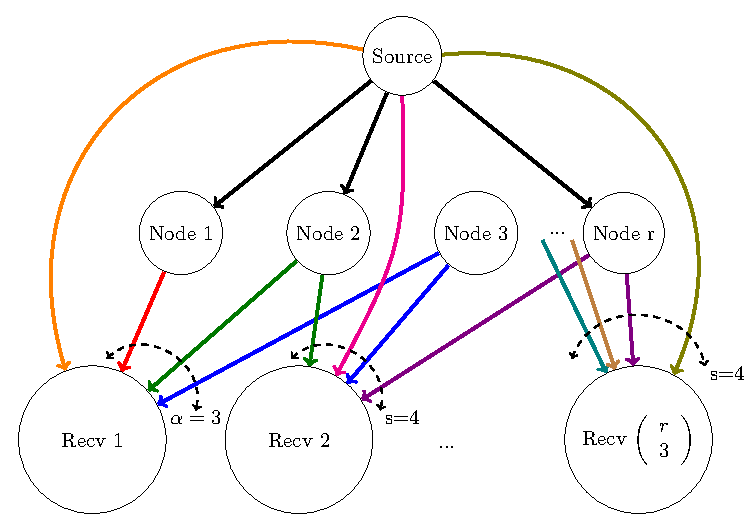
\includegraphics[width=0.5\paperwidth]{./figures/nw_e1_l1_h3_r_s4}
\end{figure}

In this subsection, we derive a lower bound on the maximum number
of receivers for the $\left(\epsilon=1,\ell=1\right)-\mathcal{N}_{h=3,r,s=4}$
network such that a vector solution for the network exists. Due to
$\alpha=3$, the number of receivers is $N=\left(\begin{array}{c}
r\\
3
\end{array}\right)$ by definition in Section \ref{sec:Description_GCN}. A problem of
finding the maximum $N$ is thus equivalent to find a maximum number
of intermediate nodes $r$. We denote the maximum number of such nodes
for a vector solution by $r_{\mathrm{max,vector}}$. Our goal is therefore
to derive $r_{\mathrm{max,vector}}$ such that there exists a vector
solution for the $\left(1,1\right)-\mathcal{N}_{3,r,4}$ network for
any $r\leq r_{\mathrm{max,vector}}$. In \cite[Section VIII.C]{Wachter-Zeh:2018},
Etzion and Wachter-Zeh stated that there exists a scalar solution
for the network for any $r\leq r_{\mathrm{max,scalar}}$ with $r_{\mathrm{max,scalar}}=2\left(q_{s}^{2}+q_{s}+1\right)$.
Based on $r_{\mathrm{max,scalar}}$ and $r_{\mathrm{max,vector}}$,
we then calculate the gap in alphabet sizes for such scalar and vector
solutions of the $\left(1,1\right)-\mathcal{N}_{3,r,4}$ network following
to Section \ref{subsec:Comparison-between-scalar-and-vector-sol}.
To discuss the vector solvability of the network, we introduce a rank
requirement on the transfer matrix $\boldsymbol{A}_{j}$ corresponding
to each receiver $R_{j}$. In Figure \ref{fig:nw_e1_l1_h3_r_s4},
each receiver $R_{j}$ obtains 4 linear combinations of the 3 source
messages. In other words, the transfer matrix $\boldsymbol{A}_{j}$
maps the messages $x_{1},x_{2},x_{3}$ to $y_{j}^{\left(1\right)},y_{j}^{\left(2\right)},y_{j}^{\left(3\right)},y_{j}^{\left(4\right)}$
or $\boldsymbol{x}_{1},\boldsymbol{x}_{2},\boldsymbol{x}_{3}$ to
$\boldsymbol{y}_{j}^{\left(1\right)},\boldsymbol{y}_{j}^{\left(2\right)},\boldsymbol{y}_{j}^{\left(3\right)},\boldsymbol{y}_{j}^{\left(4\right)}$
respectively regarding to scalar or vector network coding, which are
illustrated as linear systems of equations for $R_{1}$ in Figure
\ref{fig:rk_h3}. Both $r_{\mathrm{scalar}}$ and $r_{\mathrm{vector}}$
indicate the number of nodes $r$ and we mostly use $r$ in this subsection
for ease of notation.

\begin{figure}[H]
\caption{The vector network coding of $(\epsilon=1,l=1)-\mathcal{N}_{h=3,r,s=4}$
represents as a matrix problem \label{fig:rk_h3}}

\centering{}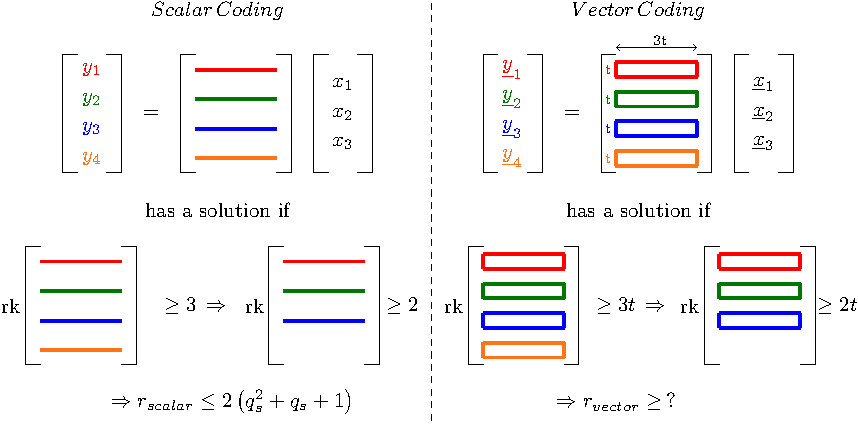
\includegraphics[width=0.6\paperwidth]{./figures/rk_h3}
\end{figure}

Following to (\ref{eq:linear_system}), each receiver $R_{j}$ has
to solve a linear equation system of $3t$ variables with $4t$ equations
to recover $h=3$ messages as below:
\begin{equation}
\left[\begin{array}{c}
\boldsymbol{y}_{j}^{\left(1\right)}\\
\boldsymbol{y}_{j}^{\left(2\right)}\\
\boldsymbol{y}_{j}^{\left(3\right)}\\
\boldsymbol{y}_{j}^{\left(4\right)}
\end{array}\right]=\boldsymbol{A}_{j}\cdot\underline{x}=\left[\begin{array}{c}
\boldsymbol{A}^{\left(r_{1}\right)}\\
\boldsymbol{A}^{\left(r_{2}\right)}\\
\boldsymbol{A}^{\left(r_{3}\right)}\\
\boldsymbol{B}^{\left(j\right)}
\end{array}\right]\cdot\left[\begin{array}{c}
\boldsymbol{x}_{1}\\
\boldsymbol{x}_{2}\\
\boldsymbol{x}_{3}
\end{array}\right],\label{eq:linear_system_h3rs4}
\end{equation}
with $\boldsymbol{x}_{1},\ldots,\boldsymbol{x}_{3}\in\ensuremath{\mathbb{F}}_{q}^{t},\boldsymbol{y}_{j}^{\left(1\right)},\ldots,\boldsymbol{y}_{j}^{\left(4\right)}\in\ensuremath{\mathbb{F}}_{q}^{t},\boldsymbol{A}^{\left(r_{v}\right)},\in\ensuremath{\mathbb{F}}_{q}^{t\times3t}$
for $v=1,\ldots,3$ and $1\leq r_{1}<r_{2}<r_{3}\leq r$, and $\boldsymbol{B}^{\left(j\right)}\in\ensuremath{\mathbb{F}}_{q}^{t\times3t}$
for $j\in\left\{ 1,\ldots,\left(\begin{array}{c}
r\\
3
\end{array}\right)\right\} $.

The network is solvable, if $\boldsymbol{A}_{j}$ has full rank as
following,
\[
\mathrm{rk}\left[\begin{array}{c}
\boldsymbol{A}_{j}^{\left(r_{1}\right)}\\
\boldsymbol{A}_{j}^{\left(r_{2}\right)}\\
\boldsymbol{A}_{j}^{\left(r_{3}\right)}\\
\boldsymbol{B}^{\left(j\right)}
\end{array}\right]\geq3t.
\]

Since coding coefficients for $\boldsymbol{B}^{\left(j\right)}$ can
be independently chosen for any receiver $R_{j}$, there always exists
$\boldsymbol{B}^{\left(j\right)}$ such that
\begin{equation}
\mathrm{rk}\left[\begin{array}{c}
\boldsymbol{A}^{\left(r_{1}\right)}\\
\boldsymbol{A}^{\left(r_{2}\right)}\\
\boldsymbol{A}^{\left(r_{3}\right)}
\end{array}\right]\geq2t,\label{eq:rk_rqm_e1l1h3s4}
\end{equation}
if and only if $\mathrm{rk}\left[\boldsymbol{A}_{j}\right]\geq3t$.

We formalize the problem by an approach with Lov\'asz local lemma,
which was initially proposed by Schwartz in \cite{MosheSchwartz:2018}.

Let $\mathcal{E}_{r_{1},r_{2},r_{3}}$ be an event that a receiver
$R_{j}$ is assigned a transfer matrix $\boldsymbol{A}_{j}$ such that
$\mathrm{rk}\left[\begin{array}{c}
\boldsymbol{A}^{\left(r_{1}\right)}\\
\boldsymbol{A}^{\left(r_{2}\right)}\\
\boldsymbol{A}^{\left(r_{3}\right)}
\end{array}\right]<2t$, i.e.,

\[
\mathcal{E}_{r_{1},r_{2},r_{3}}=\left\{ \mathrm{rk}\left[\begin{array}{c}
\boldsymbol{A}^{\left(r_{1}\right)}\\
\boldsymbol{A}^{\left(r_{2}\right)}\\
\boldsymbol{A}^{\left(r_{3}\right)}
\end{array}\right]<2t\right\} ,
\]

for $1\leq r_{1}<r_{2}<r_{3}\leq r$ and $\boldsymbol{A}^{\left(r_{1}\right)},\ldots,\boldsymbol{A}^{\left(r_{3}\right)}\in\ensuremath{\mathbb{F}}_{q}^{t\times3t}$,
chosen idenpendently and uniformly random.
\begin{lem}[Symmetric Lov\'asz local lemma (LLL) \cite{Schwarz:2013}]
 A set of events $\mathcal{E}_{i}$, such that each event occurs
with probability at most $p$. If each event is independent of all
others except for at most $d$ of them and $4pd\leq1$, then: $\mathrm{Pr}\left[\stackrel[i=1]{n}{\bigcap}\overline{\mathcal{E}}_{i}\right]>0$.
\label{thm:LLL}
\end{lem}
In \cite{Overbeck:2007}, the number of $\left[n\times m\right]$
matrices of rank $i$ over $\ensuremath{\mathbb{F}}_{q}$ is given,

\begin{equation}
\mathrm{NM}_{i,n,m}=\stackrel[j=0]{i-1}{\mathop{\prod}}\frac{\left(q^{m}-q^{j}\right)\left(q^{n}-q^{j}\right)}{q^{i}-q^{j}}.\label{eq:num_of_rank_t_matrices}
\end{equation}

We therefore have $\mathrm{NM}_{i<2t,3t,3t}$ as the number of $\left[3t\times3t\right]$
matrices whose ranks are less than $2t$. Each event $\mathcal{E}_{r_{1},r_{2},r_{3}}$
has a probability calculated by dividing $\mathrm{NM}_{i<2t,3t,3t}$
by $q^{9t^{2}}$, where $q^{9t^{2}}$ is the number of all possible
$\left[3t\times3t\right]$ matrices over $\ensuremath{\mathbb{F}}_{q}$.
The probability is bounded as stated in Lemma \ref{lem:prob_p_LLL_formula}.
\begin{lem}
\label{lem:prob_p_LLL_formula} If $\mathrm{Pr}\left[\mathcal{E}_{r_{1},r_{2},r_{3}}\right]\leq p$,
then,
\[
p\in\Theta\left(q^{-t^{2}-2t-1}\right),\forall t\geq2.
\]
\end{lem}
\begin{proof}
Following to (\ref{eq:rk_rqm_e1l1h3s4}), a event $\mathcal{E}_{r_{1},r_{2},r_{3}}$
occurs when $\mathrm{rk}\left[\boldsymbol{A}_{j}\right]<3t$, and
its probability is bounded by $p$ (with $0\leq p\leq1$) as following,
\begin{eqnarray}
\mathrm{Pr}\left[\mathcal{E}_{r_{1},r_{2},r_{3}}\right]=\mathrm{Pr}\left[\mathrm{rk}\left[\begin{array}{c}
\boldsymbol{A}^{\left(r_{1}\right)}\\
\boldsymbol{A}^{\left(r_{2}\right)}\\
\boldsymbol{A}^{\left(r_{3}\right)}
\end{array}\right]<2t\right] & = & \stackrel[i=0]{2t-1}{\mathop{\sum}}\mathrm{Pr}\left[\mathrm{rk}\left[\begin{array}{c}
\boldsymbol{A}_{j}^{\left(r_{1}\right)}\\
\boldsymbol{A}_{j}^{\left(r_{2}\right)}\\
\boldsymbol{A}_{j}^{\left(r_{3}\right)}
\end{array}\right]=i\right]\label{eq:p_in_LLL}\\
 & \overset{1}{=} & \stackrel[i=0]{2t-1}{\mathop{\sum}}\frac{\mathrm{NM}_{i,3t,3t}}{q^{\left(3t\right)\cdot\left(3t\right)}}\nonumber \\
 & = & \stackrel[i=0]{2t-1}{\mathop{\sum}}\frac{\stackrel[j=0]{i-1}{\mathop{\prod}}\frac{\left(q^{3t}-q^{j}\right)^{2}}{q^{i}-q^{j}}}{q^{9t^{2}}}.\label{eq:p_eq_h3}
\end{eqnarray}

(1): Applying (\ref{eq:num_of_rank_t_matrices}) for $\left[3t\times3t\right]$
matrices over $\ensuremath{\mathbb{F}}_{q}$ of rank $i=0,\ldots,2t-1$.

In the following, we view $\stackrel[j=0]{i-1}{\mathop{\prod}}\frac{\left(q^{3t}-q^{j}\right)^{2}}{q^{i}-q^{j}}$
as a polynomial in $q$.

We consider the numerator of (\ref{eq:p_eq_h3}): $\stackrel[j=0]{i-1}{\mathop{\prod}}\frac{\left(q^{3t}-q^{j}\right)^{2}}{q^{i}-q^{j}}=\frac{p_{N}^{(i)}(q)}{p_{D}^{(i)}(q)}=p^{(i)}(q)$.

Due to $i$-times product and large $t$: $\left.\begin{array}{c}
\mathrm{deg}\left(p_{N}^{(i)}(q)\right)=q^{i6t}\\
\mathrm{deg}\left(p_{D}^{(i)}(q)\right)=q^{i^{2}}
\end{array}\right\} \Rightarrow p^{(i)}(q)\approx q^{i6t-i^{2}}$.

Therefore, we have: $\stackrel[i=0]{2t-1}{\mathop{\sum}}\stackrel[j=0]{i-1}{\mathop{\prod}}\frac{\left(q^{3t}-q^{j}\right)^{2}}{q^{i}-q^{j}}=\stackrel[i=0]{2t-1}{\mathop{\sum}}p^{(i)}(q)\approx\stackrel[i=0]{2t-1}{\mathop{\sum}}q^{i6t-i^{2}}$.

To maximize the sum, we set derivation of it to 0 and find the corresponding
root: 
\begin{eqnarray*}
 & \left(i6t-i^{2}\right)^{'} & =0\\
\Leftrightarrow & 6t-2i & =0\\
\Leftrightarrow & i & =3t.
\end{eqnarray*}

However, the upper limit of the sum is $\left(2t-1\right)$, which
is less than $3t$ for all $t\geq2$.
\[
\Rightarrow\mathrm{max}\left\{ q^{i6t-i^{2}}:i=0,2\ldots,2t-1\right\} =\left.q^{i6t-i^{2}}\right|_{i=2t-1}=q^{8t^{2}-2t-1}.
\]

Hence,
\[
\underset{i}{\mathrm{max}}\left\{ \stackrel[i=0]{2t-1}{\mathop{\sum}}p^{(i)}(q)\right\} \in\Theta\left(\mathrm{max}\left\{ q^{i6t-i^{2}}:i=1,2\ldots,2t-1\right\} \right)=\Theta\left(q^{8t^{2}-2t-1}\right)
\]
\[
\Rightarrow\underset{i}{\mathrm{max}}\left\{ \frac{\stackrel[i=0]{2t-1}{\mathop{\sum}}p^{(i)}(q)}{q^{9t^{2}}}\right\} \in\Theta\left(q^{-t^{2}-2t-1}\right)
\]
\[
\Rightarrow p\in\Theta\left(q^{-t^{2}-2t-1}\right)
\]
\end{proof}
Each event considered under the Lov\'asz Local Lemma \ref{thm:LLL}
is not required to be independent to all other events, and it allows
some dependence among events stated in Lemma \ref{lem:dependecy_d_LLL}.
\begin{lem}
Each event $\mathcal{E}_{r_{1},r_{2},r_{3}}$ is dependent on at most
$d\left(r\right)\leq\frac{3}{2}r^{2}$ other events. \label{lem:dependecy_d_LLL}
\end{lem}
\begin{proof}
It is clear that $\mathcal{E}_{r_{1},r_{2},r_{3}}$ is dependent on
$\mathcal{E}_{r_{1}^{'},r_{2}^{'},r_{3}^{'}}$ if and only if $\left\{ r_{1},r_{2},r_{3}\right\} \cap\left\{ r_{1}^{'},r_{2}^{'},r_{3}^{'}\right\} \neq\emptyset$.
Let us consider $\left\{ r_{1},r_{2},r_{3}\right\} \cap\left\{ r_{1}^{'},r_{2}^{'},r_{3}^{'}\right\} =\left\{ r_{1}\right\} =\left\{ r_{1}^{'}\right\} $,
we have maximum $\left(\begin{array}{c}
r-1\\
2
\end{array}\right)$ such $\mathcal{E}_{r_{1},r_{2},r_{3}}$ events. Similarly with $\left\{ r_{1},r_{2},r_{3}\right\} \cap\left\{ r_{1}^{'},r_{2}^{'},r_{3}^{'}\right\} =\left\{ r_{2}\right\} $
and $\left\{ r_{1},r_{2},r_{3}\right\} \cap\left\{ r_{1}^{'},r_{2}^{'},r_{3}^{'}\right\} =\left\{ r_{3}\right\} $,
we obtain
\[
d\left(r\right)\leq3\cdot\left(\begin{array}{c}
r-1\\
2
\end{array}\right)=3\cdot\frac{\left(r-1\right)\left(r-2\right)}{2}=\frac{3}{2}\left(r^{2}-3r+2\right)
\]
\[
\Rightarrow d\left(r\right)\leq\frac{3}{2}r^{2}
\]

Therefore, each event $\mathcal{E}_{r_{1},r_{2},r_{3}}$ is independent
of all other events except at most $d\leq\frac{3}{2}r^{2}$ of them.
\end{proof}
\begin{thm}
There is an $r_{\mathrm{max,vector}}\in\Omega\left(q^{t^{2}/2+\mathcal{O}\left(t\right)}\right)$
such that for any $r\leq r_{\mathrm{max,vector}}$ there exists a
vector solution for the $\left(\epsilon=1,l=1\right)-\mathcal{N}_{h=3,r,s=4}$
network . \label{theo:r_for_vector_sol_e1l1h3rs4}
\end{thm}
\begin{proof}
By the intersection rule, none of the $\mathcal{E}_{r_{1},r_{2},r_{3}}$
events occuring is equivalent to an event $T$ whose set of outcomes
satisfy (\ref{eq:rk_rqm_e1l1h3s4}) as following,
\[
T=\stackrel[i=1]{n}{\bigcap}\overline{\mathcal{E}}_{i}=\left\{ \mathrm{rk}\left[\begin{array}{c}
\boldsymbol{A}^{\left(r_{1}\right)}\\
\boldsymbol{A}^{\left(r_{2}\right)}\\
\boldsymbol{A}^{\left(r_{3}\right)}
\end{array}\right]\geq2t,\forall1\leq r_{1}<r_{2}<r_{3}\leq r\right\} .
\]
The Lov\'asz Local Lemma \ref{thm:LLL} shows that $\mathrm{Pr}\left[T\right]=\mathrm{Pr}\left[\stackrel[i=1]{n}{\bigcap}\overline{\mathcal{E}}_{i}\right]>0$
if $4\cdot p\cdot d(r)\leq1,\forall r\leq r_{\mathrm{max,vector}}$.
Furthermore, we have $d\leq\frac{3}{2}r^{2}$ following to Lemma \ref{lem:dependecy_d_LLL},
which gives: $4\cdot p\cdot\frac{3}{2}r^{2}\leq1\Rightarrow r\leq\sqrt{\frac{1}{6p}}=r_{\mathrm{max,vector}}$.

By Lemma \ref{lem:prob_p_LLL_formula}, we have $p\in\Theta\left(q^{-t^{2}-2t-1}\right)$,
\[
\Rightarrow r_{\mathrm{max,vector}}\in\Omega\left(\sqrt{\frac{1}{6p}}\right)=\Omega\left(\sqrt{\frac{1}{6q^{-t^{2}-2t-1}}}\right)=\Omega\left(q^{t^{2}/2+\mathcal{O}\left(t\right)}\right).
\]
The sufficient condition of Lemma \ref{thm:LLL} is satisfied for
any $r\leq r_{\mathrm{max,vector}}\in\Omega\left(q^{t^{2}/2+\mathcal{O}\left(t\right)}\right)$.
None of the $\mathcal{E}_{r_{1},r_{2},r_{3}}$ events occurs, so there
exists a vector solution for such $r$.
\end{proof}
\begin{cor}
The $\left(\epsilon=1,\ell=1\right)-\mathcal{N}_{h=3,r,s=4}$ network
has a vector solution with a gap $q^{t^{2}/4+\mathcal{O}(t)}$.
\end{cor}
\begin{proof}
In \cite[Sec. VIII-C]{Wachter-Zeh:2018}, we have that $r_{\mathrm{max,scalar}}\in\mathcal{O}\left(q_{\mathrm{s}}^{2}\right)$,
where they proved that
\begin{equation}
r_{\mathrm{scalar}}\leq2\left[\begin{array}{c}
3\\
1
\end{array}\right]_{q_{\mathrm{s}}}=2\left(q_{\mathrm{s}}^{2}+q_{\mathrm{s}}+1\right).\label{eq:r_scalar_max}
\end{equation}
Following to Section \ref{subsec:Comparison-between-scalar-and-vector-sol}
and Theorem \ref{theo:r_for_vector_sol_e1l1h3rs4}, we have the gap
size 
\begin{eqnarray}
 & r_{\mathrm{max,scalar}} & =r_{\mathrm{max,vector}}\nonumber \\
\Leftrightarrow & q_{\mathrm{s,min,from\,bound}}^{2} & =q^{t^{2}/2+\mathcal{O}(t)}\nonumber \\
\Leftrightarrow & q_{\mathrm{s,min,from\,bound}} & ^{=}q^{t^{2}/4+\mathcal{O}(t)}\nonumber \\
\Rightarrow & g_{\mathrm{lower\,bound}} & =q_{\mathrm{s,min,from\,bound}}-q_{v}=q^{t^{2}/4+\mathcal{O}(t)}\label{eq:gap_e1l1h3rs4}
\end{eqnarray}

Therefore, there exists a vector solution for the network to achieve
such gap.
\end{proof}
\begin{table}[H]
\begin{centering}
\begin{tabular}{|c|c|c|}
\hline 
t & Scalar Solution & Vector Solution\tabularnewline
\hline 
\hline 
2 & $r_{\mathrm{max,scalar}}=42$ & $r_{\mathrm{max,vector}}\geq7$\tabularnewline
\hline 
3 & $r_{\mathrm{max,scalar}}=146$ & $r_{\mathrm{max,vector}}\geq62$ \tabularnewline
\hline 
4 & $r_{\mathrm{max,scalar}}=546$ & $r_{\mathrm{max,vector}}\geq1317$\tabularnewline
\hline 
5 & $r_{\mathrm{max,scalar}}=2114$ & $r_{\mathrm{max,vector}}\geq58472$\tabularnewline
\hline 
6 & $r_{\mathrm{max,scalar}}=8322$ & $r_{\mathrm{max,vector}}>10^{6}$\tabularnewline
\hline 
\end{tabular}
\par\end{centering}
\centering{}\caption{Number of intermediate nodes $r$ for the $\left(\epsilon=1,\ell=1\right)-\mathcal{N}_{h=3,r,s=4}$
network such that scalar and vector solutions exist over $t=2,\ldots,6$.
Following to (\ref{eq:r_scalar_max}), there exists a scalar solution
for the network if and only if $r\protect\leq2\left(q_{s}^{2}+q_{s}+1\right)=r_{\mathrm{max,scalar}}$.
Following to (\ref{eq:p_eq_h3}) and Lemma \ref{lem:dependecy_d_LLL},
we observed that vector solutions outperforming the scalar solution
when $t\protect\geq4$. \label{tab:r_over_t}}
\end{table}

By varying $t$ in (\ref{eq:p_eq_h3}), we have the Table \ref{tab:r_over_t}.
In the Table \ref{tab:r_over_t}, the vector solution outperforms
the scalar solution when $t\geq4$ for the network $\left(\epsilon=1,\ell=1\right)-\ensuremath{N}_{h=3,r,s=4}$.
In Section \ref{sec:Main-Approach} and Section \ref{sec:Alternative-Approaches}
for computational results of the network, we show vector solutions
outperforming scalar solutions in case of $t=2$ and $t=3$.

\section{$\left(\epsilon=1,\ell=1\right)-\mathcal{N}_{h,r,s}$ Network \label{sec:e1l1_nw}}

The $\left(\epsilon=1,\ell=1\right)-\mathcal{N}_{h,r,s}$ network
is a more general network compared to the $\left(\epsilon=1,\ell=1\right)-\mathcal{N}_{3,r,4}$
network studied in the previous subsection. We study a gap between
scalar and vector solutions for the $\left(1,1\right)-\mathcal{N}_{h,r,s}$
network by deriving a lower bound on the maximum number of intermediate
nodes $r$. Following to (\ref{eq:linear_system}) and an extension
of (\ref{eq:linear_system_h3rs4}), each receiver $R_{j}$ has to
solve a linear equation of $ht$ variables with $st$ equations to
recover $h$ messages as following,

\[
\left[\begin{array}{c}
\boldsymbol{y}_{j}^{\left(1\right)}\\
\vdots\\
\boldsymbol{y}_{j}^{\left(\alpha\right)}\\
\boldsymbol{y}_{j}^{\left(\alpha+1\right)}
\end{array}\right]=\boldsymbol{A}_{j}\cdot\underline{x}=\left[\begin{array}{c}
\boldsymbol{A}^{\left(r_{1}\right)}\\
\vdots\\
\boldsymbol{A}^{\left(r_{\alpha}\right)}\\
\boldsymbol{B}^{\left(j\right)}
\end{array}\right]\cdot\left[\begin{array}{c}
\boldsymbol{x}_{1}\\
\vdots\\
\boldsymbol{x}_{h}
\end{array}\right],
\]

with $\boldsymbol{x}_{1},\ldots,\boldsymbol{x}_{h}\in\ensuremath{\mathbb{F}}_{q}^{t},\boldsymbol{y}_{j}^{\left(1\right)},\ldots,\boldsymbol{y}_{j}^{\left(\alpha+1\right)}\in\ensuremath{\mathbb{F}}_{q}^{t},\boldsymbol{A}^{\left(r_{1}\right)},\ldots,\boldsymbol{A}^{\left(r_{\alpha}\right)}\in\ensuremath{\mathbb{F}}_{q}^{t\times ht}$
for $1\leq r_{1}<\ldots<r_{\alpha}\leq r$, $\boldsymbol{B}^{\left(j\right)}\in\ensuremath{\mathbb{F}}_{q}^{t\times ht}$
for $j\in\left\{ 1,\ldots,\left(\begin{array}{c}
r\\
\alpha
\end{array}\right)\right\} $.

Since coding coefficients for $\boldsymbol{B}^{\left(j\right)}$ can
be independently chosen for any receiver $R_{j}$, there always exists
$\boldsymbol{B}^{\left(j\right)}$ such that the network is solvable
with 
\[
\mathrm{rk}\left[\begin{array}{c}
\boldsymbol{A}^{\left(r_{1}\right)}\\
\vdots\\
\boldsymbol{A}^{\left(r_{\alpha}\right)}
\end{array}\right]\geq ht-t,
\]

if and only if the transfer matrix $\boldsymbol{A}_{j}$ has full
rank.

Similar to $\left(1,1\right)-\ensuremath{N}_{3,r,4}$, we apply the
Lov\'asz Local Lemma \ref{thm:LLL} for the following $\mathcal{E}_{r_{1},\ldots,r_{h-\epsilon}}$
to study the gap between scalar and vector solutions for the $\left(1,1\right)-\mathcal{N}_{h,r,s}$
network.

Let $\mathcal{E}_{r_{1},\ldots,r_{\alpha}}$ be an event that a receiver
$R_{j}$ is assigned a transfer matrix $\boldsymbol{A}_{j}$ such
that $\mathrm{rk}\left[\begin{array}{c}
\boldsymbol{A}^{\left(r_{1}\right)}\\
\vdots\\
\boldsymbol{A}^{\left(r_{\alpha}\right)}
\end{array}\right]<(h-1)t$, i.e.,

\[
\mathcal{E}_{r_{1},\ldots,r_{\alpha}}=\left\{ \mathrm{rk}\left[\begin{array}{c}
\boldsymbol{A}^{\left(r_{1}\right)}\\
\vdots\\
\boldsymbol{A}^{\left(r_{\alpha}\right)}
\end{array}\right]<(h-1)t\right\} ,
\]

for $1\leq r_{1}<\ldots<r_{\alpha}\leq r$ and $\boldsymbol{A}^{\left(r_{1}\right)},\ldots,\boldsymbol{A}^{\left(r_{\alpha}\right)}\in\ensuremath{\mathbb{F}}_{q}^{t\times ht}$,
chosen independently and uniformly random.
\begin{lem}
\label{lem:p_e1l1}If $\mathrm{Pr}\left[\mathcal{E}_{r_{1},\ldots,r_{\alpha}}\right]\leq p$,
then,
\[
p\in\Theta\left(q^{\left(h-\alpha\right)t^{2}+\mathcal{O}(t)}\right),\forall t\geq2.
\]
\end{lem}
\begin{proof}
The probability of an event $\mathcal{E}_{r_{1},\ldots,r_{\alpha}}$
can be calculated by 

\begin{eqnarray}
\mathrm{Pr}\left[\mathcal{E}_{r_{1},\ldots,r_{\alpha}}\right] & = & \stackrel[i=0]{(h-1)t-1}{\mathop{\sum}}\mathrm{Pr}\left[\mathrm{rk}\left[\begin{array}{c}
\boldsymbol{A}^{\left(r_{1}\right)}\\
\vdots\\
\boldsymbol{A}^{\left(r_{\alpha}\right)}
\end{array}\right]=i\right]\nonumber \\
 & \overset{1}{=} & \stackrel[i=0]{(h-1)t-1}{\mathop{\sum}}\frac{\mathrm{NM}_{i,\alpha t,ht}}{q^{\left(\alpha t\right)\left(ht\right)}}\nonumber \\
 & = & \frac{1}{q^{\left(\alpha h\right)t^{2}}}\cdot\stackrel[i=0]{(h-1)t-1}{\mathop{\sum}}\stackrel[j=0]{i-1}{\mathop{\prod}}\frac{\left(q^{\alpha t}-q^{j}\right)\left(q^{ht}-q^{j}\right)}{q^{i}-q^{j}}.\label{eq:general_nw_calc_p}
\end{eqnarray}

(1): The formula for the number of $\left[\alpha t\times ht\right]$
matrices of rank $i$ over $\ensuremath{\mathbb{F}}_{q}$ was introduced
in the previous subsection as (\ref{eq:num_of_rank_t_matrices}).

We consider firstly the product $\stackrel[j=0]{i-1}{\mathop{\prod}}\frac{\left(q^{\alpha t}-q^{j}\right)\left(q^{ht}-q^{j}\right)}{q^{i}-q^{j}}$
as a polynomial in $q$, then we have

\[
\stackrel[j=0]{i-1}{\mathop{\prod}}\frac{\left(q^{\alpha t}-q^{j}\right)\left(q^{ht}-q^{j}\right)}{q^{i}-q^{j}}=\frac{p_{N}^{(i)}(q)}{p_{D}^{(i)}(q)}=p^{(i)}(q).
\]

For $t\rightarrow\infty$: $\left.\begin{array}{c}
\mathrm{deg}\left(p_{N}^{(i)}(q)\right)=q^{i(\alpha t+ht)}\\
\mathrm{deg}\left(p_{D}^{(i)}(q)\right)=q^{i^{2}}
\end{array}\right\} \Rightarrow p^{(i)}(q)\approx q^{i(\alpha t+ht)-i^{2}}.$

Now, we evaluate the function $f(i)=i(\alpha t+ht)-i^{2}$ to find
its maximum point by its derivation, 

$f'(i^{*})=0\Leftrightarrow(\alpha t+ht)-2i^{*}=0\Leftrightarrow i^{*}=\frac{\alpha t+ht}{2}.$

Considering the sum $\stackrel[i=0]{(h-1)t-1}{\mathop{\sum}}p^{(i)}(q)$,
we have to check whether the point $i^{*}$ in $\left\{ 0,\ldots,(h-1)t-1\right\} $.
For the lower bound, we need $0\leq i^{*}\Leftrightarrow0\leq\frac{\alpha t+ht}{2}\Leftrightarrow t\geq\frac{2}{\alpha+h}$,
which is always true due to the given $t\geq2$ and $\alpha,h\geq3$
following to Theorem \ref{nw_parameters}.

Regarding to the upper bound, we need $\frac{\alpha t+ht}{2}\leq(h-1)t-1\Leftrightarrow t\leq\frac{-2}{\alpha+2-h}$.
Furthermore, we always have $\alpha+2>h$ due to $\alpha l+\epsilon=\alpha+1\geq h$
by Theorem \ref{nw_parameters}. Thus we need $t<0$ for $i^{*}\in\left\{ 0,\ldots,(h-1)t-1\right\} $,
which cannot happen since we always have $t\geq2$ for a vector solution.
For $i\in\left\{ 0,\ldots,(h-1)t-1\right\} $, the maximum value of
$q^{i(\alpha t+ht)-i^{2}}$ is therefore as following,
\begin{eqnarray*}
\mathrm{max}\left\{ q^{i(\alpha t+ht)-i^{2}}:i=0,\ldots,(h-1)t-1\right\}  & = & \left.q^{i(\alpha t+ht)-i^{2}}\right|_{i=(h-1)t-1}\\
 & = & q^{\left[\left(h-1\right)\left(\alpha+1\right)\right]t^{2}-\left(\alpha-h+2\right)t-1}.
\end{eqnarray*}

Secondly, we apply the maximum value to the sum, we have:
\begin{eqnarray*}
 & \mathrm{max}\left\{ \stackrel[i=0]{(h-1)t-1}{\mathop{\sum}}p^{(i)}(q)\right\}  & \in\Theta\left(q^{\left[\left(h-1\right)\left(\alpha+1\right)\right]t^{2}+\mathcal{O}(t)}\right)\\
\Rightarrow & \mathrm{max}\left\{ \frac{\stackrel[i=0]{(h-1)t-1}{\mathop{\sum}}p^{(i)}(q)}{q^{\left(\alpha h\right)t^{2}}}\right\}  & \in\Theta\left(\frac{q^{\left[\left(h-1\right)\left(\alpha+1\right)\right]t^{2}+\mathcal{O}(t)}}{q^{\left(\alpha h\right)t^{2}}}\right)
\end{eqnarray*}
\[
\Rightarrow p\in\Theta\left(q^{\left(h-\alpha-1\right)t^{2}+\mathcal{O}(t)}\right)
\]

Therefore, we have that each event $\mathcal{E}_{r_{1},\ldots,r_{\alpha}}$
 occurs with probability at most $p\in\Theta\left(q^{\left(h-\alpha-1\right)t^{2}+\mathcal{O}(t)}\right)$.
\end{proof}
\begin{lem}
Each event $\mathcal{E}_{r_{1},\ldots,r_{h-\epsilon}}$ is dependent
for at most $d\left(r\right)\leq\frac{\alpha}{\left(\alpha-1\right)!}r^{^{\alpha-1}}$
other events. \label{lem:d_e1l1}
\end{lem}
\begin{proof}
Similar to $\left(\epsilon=1,\ell=1\right)-\ensuremath{N}_{3,r,4}$,
we have:
\[
d\leq\alpha\left(\begin{array}{c}
r-1\\
\alpha-1
\end{array}\right)=\alpha\frac{\left(r-1\right)\ldots\left(r-\alpha+1\right)}{\left(\alpha-1\right)!}\leq\frac{\alpha}{\left(\alpha-1\right)!}r^{^{\alpha-1}}
\]
\end{proof}
\begin{thm}
There is $r_{\mathrm{max,vector}}\in\Omega\left(q^{\frac{h-\alpha-1}{1-\alpha}t^{2}+\mathcal{O}(t)}\right)$
such that for any $r\leq r_{\mathrm{max,vector}}$ there exists a
vector solution for the $\left(\epsilon=1,\ell=1\right)-\ensuremath{N}_{h,r,s}$
network. \label{theo:r_vector_e1l1}
\end{thm}
\begin{proof}
Following to the Lov\'asz Local Lemma \ref{thm:LLL} and Lemma \ref{lem:d_e1l1},
there exists a vector solution for the network if $4dp\leq1\Rightarrow d\leq\frac{\alpha}{\left(\alpha-1\right)!}r^{^{\alpha-1}}\Rightarrow r\leq\left(\frac{\left(\alpha-1\right)!}{4\alpha}\cdot\frac{1}{p}\right)^{\frac{1}{\alpha-1}}=r_{\mathrm{max,vector}}$.
By Lemma \ref{lem:d_e1l1}, we further have $p\in\Theta\left(q^{\left(h-\alpha-1\right)t^{2}+\mathcal{O}(t)}\right),\forall t\geq2$
as an upper bound of $\mathrm{Pr}\left[\mathcal{E}_{r_{1},\ldots,r_{\alpha}}\right]$.
Applying such $p$ to $r_{\mathrm{max,vector}}$, we therefore have
$r_{\mathrm{max,vector}}\in\Omega\left(q^{\frac{h-\alpha-1}{1-\alpha}t^{2}+\mathcal{O}(t)}\right)$.

Hence, the sufficient condition of the Local lemma \ref{thm:LLL}
is satisfied for any $r\leq r_{\mathrm{max,vector}}\in\Omega\left(q^{\frac{h-\alpha-1}{1-\alpha}t^{2}+\mathcal{O}(t)}\right)$
and a vector solution exists for such $r$.
\end{proof}
To calculate the gap, we then study scalar solutions for the $\left(1,1\right)-\ensuremath{N}_{h,r,s}$
network. Following to (\ref{eq:linear_system}) for a scalar solution,
each receiver $R_{j}$ have to solve the following linear system to
reconstruct its requested messages,

\[
\left[\begin{array}{c}
y_{j}^{\left(1\right)}\\
\vdots\\
y_{j}^{\left(\alpha\right)}\\
y_{j}^{\left(\alpha+1\right)}
\end{array}\right]=\left[\begin{array}{c}
\boldsymbol{a}^{\left(r_{1}\right)}\\
\vdots\\
\boldsymbol{a}^{\left(r_{\alpha}\right)}\\
\boldsymbol{b}^{\left(j\right)}
\end{array}\right]\cdot\left[\begin{array}{c}
x_{1}\\
\vdots\\
x_{h}
\end{array}\right],
\]

with $x_{1},\ldots,x_{h}\in\ensuremath{\mathbb{F}}_{q_{\mathrm{s}}},y_{j}^{\left(1\right)},\ldots,y_{j}^{\left(\alpha+1\right)}\in\ensuremath{\mathbb{F}}_{q_{\mathrm{s}}},\boldsymbol{a}^{\left(r_{1}\right)},\ldots,\boldsymbol{a}^{\left(r_{\alpha}\right)}\in\ensuremath{\mathbb{F}}_{q_{\mathrm{s}}}^{h}$
for $1\leq r_{1}<\ldots<r_{\alpha}\leq r$ and $\boldsymbol{b}^{\left(j\right)}\in\ensuremath{\mathbb{F}}_{q_{\mathrm{s}}}^{h}$
for $j\in\left\{ 1,\ldots,\left(\begin{array}{c}
r\\
\alpha
\end{array}\right)\right\} $. Similar to the vector solution studied for the $\left(1,1\right)-\ensuremath{N}_{h,r,s}$
network, there exists a scalar solution if

\begin{equation}
\mathrm{rk}\left[\begin{array}{c}
\boldsymbol{a}^{\left(r_{1}\right)}\\
\vdots\\
\boldsymbol{a}^{\left(r_{\alpha}\right)}
\end{array}\right]\geq h-1.\label{eq:rk_rqm_scalar_1_1_hrs}
\end{equation}

\begin{thm}
There exists $r_{\mathrm{max,scalar}}\in\mathcal{O}\left(q_{\mathrm{s}}^{\left(\alpha-h+2\right)\left(h-2\right)}\right)$
with $\alpha\geq h\geq3$ such that for any $r\leq r_{\mathrm{max,scalar}}$
there exists a scalar solution for the $\left(\epsilon=1,\ell=1\right)-\ensuremath{N}_{h,r,s}$
network. And there exists $r_{\mathrm{max,scalar}}\in\mathcal{O}\left(q_{\mathrm{s}}^{\alpha}\right)$
with $2\leq\alpha<h$ such that for any $r\leq r_{\mathrm{max,scalar}}$
there exists a scalar solution for the $\left(\epsilon=1,\ell=1\right)-\ensuremath{N}_{h,r,s}$
network. \label{theo:r_scalar_e1l1}
\end{thm}
\begin{proof}
Following to Theorem \ref{nw_parameters}, we are interested in network
parameters satisfying $\ell+\epsilon+1\leq h\leq\alpha\ell+\epsilon$.
Given $\epsilon=1,\ell=1$, we thus consider $\alpha$ and $h$ such
that $3\leq h\leq\alpha+1$, and we distinguish the following 2 cases.

For $2\leq\alpha<h$: since $h-1\leq\alpha<h$, we have then $\alpha=h-1$.
To satisfy $\mathrm{rk}\left[\begin{array}{c}
\boldsymbol{a}^{\left(r_{1}\right)}\\
\vdots\\
\boldsymbol{a}^{\left(r_{\alpha}\right)}
\end{array}\right]\geq h-1$, all $\boldsymbol{a}^{\left(r_{1}\right)},\ldots,\boldsymbol{a}^{\left(r_{\alpha}\right)}$
must be linearly independent. The number of intermediates nodes is
thus at most the number of distinct 1-dimensional subspaces of $\ensuremath{\mathbb{F}}_{q_{\mathrm{s}}}^{h}$and
therefore, a scalar solution exists if we have

\begin{eqnarray*}
 & r & \leq\left[\begin{array}{c}
h\\
1
\end{array}\right]_{q_{\mathrm{s}}}=\left[\begin{array}{c}
\alpha+1\\
1
\end{array}\right]_{q_{\mathrm{s}}}\\
\Rightarrow & r & \leq\frac{q_{\mathrm{s}}^{\alpha+1}-1}{q_{\mathrm{s}}-1}\approx q_{\mathrm{s}}^{\alpha}\\
\Rightarrow & r_{\mathrm{max,scalar}} & \in\mathcal{O}\left(q_{\mathrm{s}}^{\alpha}\right).
\end{eqnarray*}

For $\alpha\geq h\geq3$: to ensure that each receiver receives $\alpha$
vectors $\boldsymbol{a}^{\left(r_{1}\right)},\ldots,\boldsymbol{a}^{\left(r_{\alpha}\right)}\in\ensuremath{\mathbb{F}}_{q_{\mathrm{s}}}^{h}$
which span a subspace of $\ensuremath{\mathbb{F}}_{q_{\mathrm{s}}}^{h}$
whose dimension is at least $\left(h-1\right)$, i.e. a $\mathrm{(h-1)}$-subspace
of $\ensuremath{\mathbb{F}}_{q_{\mathrm{s}}}^{h}$, we have to guarantee
that on the links between the source and the intermediate nodes, no
$\alpha$ links will contain a vector which is contained in the same
$(h-2)$-subspace ($\left(\alpha-1\right)$ such links can have such
vectors). Hence, a scalar solution exists for this case if
\begin{eqnarray*}
 & r & \leq\left(\alpha-1\right)\left[\begin{array}{c}
\alpha\\
h-2
\end{array}\right]_{q_{\mathrm{s}}}\\
\Rightarrow & r & \leq\left(\alpha-1\right)\stackrel[i=0]{h-3}{\prod}\frac{q_{\mathrm{s}}^{\alpha}-q_{\mathrm{s}}^{i}}{q_{\mathrm{s}}^{h-2}-q_{\mathrm{s}}^{i}}\approx\left(\alpha-1\right)\left(q_{\mathrm{s}}^{\left(\alpha-h+2\right)\left(h-2\right)}\right)\\
\Rightarrow & r_{\mathrm{max,scalar}} & \in\mathcal{O}\left(q_{\mathrm{s}}^{\left(\alpha-h+2\right)\left(h-2\right)}\right).
\end{eqnarray*}

Therefore, with $2\leq\alpha<h$, there exists a scalar solution for
any $r\leq r_{\mathrm{max,scalar}}\in\mathcal{O}\left(q_{\mathrm{s}}^{\alpha}\right)$
and with $\alpha\geq h\geq3$, there exists a scalar solution for
any $r\leq r_{\mathrm{max,scalar}}\in\mathcal{O}\left(q_{\mathrm{s}}^{\left(\alpha-h+2\right)\left(h-2\right)}\right)$.
\end{proof}
Following to Theorem \ref{theo:r_vector_e1l1} and Theorem \ref{theo:r_scalar_e1l1},
we compute a gap for the network in Corollary \ref{cor:gap_e1l1}.
\begin{cor}
The $\left(\epsilon=1,\ell=1\right)-\ensuremath{N}_{h,r,s}$ network
has a vector solution with a gap $q^{\frac{\alpha-h+1}{\left(\alpha-1\right)\left(\alpha-h+2\right)\left(h-2\right)}t^{2}+\mathcal{O}(t)}$.
\label{cor:gap_e1l1}
\end{cor}
\begin{proof}
Following to Section \ref{subsec:Comparison-between-scalar-and-vector-sol},

\begin{eqnarray*}
 & r_{\mathrm{max,scalar}} & =r_{\mathrm{max,vector}}\\
\Leftrightarrow & q_{\mathrm{s,min,from\,bound}}^{\left(\alpha-h+2\right)\left(h-2\right)} & =q^{\frac{h-\alpha-1}{1-\alpha}t^{2}+\mathcal{O}(t)}\\
\Leftrightarrow & q_{\mathrm{s,min,from\,bound}} & ^{=}q^{\frac{\alpha-h+1}{\left(\alpha-1\right)\left(\alpha-h+2\right)\left(h-2\right)}t^{2}+\mathcal{O}(t)}\\
\Rightarrow & g_{\mathrm{lower\,bound}} & =q_{\mathrm{s,min,from\,bound}}-q_{v}=q^{\frac{\alpha-h+1}{\left(\alpha-1\right)\left(\alpha-h+2\right)\left(h-2\right)}t^{2}+\mathcal{O}(t)}
\end{eqnarray*}

Therefore, there exists a vector solution for the network to achieve
such gap.
\end{proof}
In the next subsection, we further study the gap for a more general
network compared to the $\left(1,1\right)-\ensuremath{N}_{h,r,s}$
network.

\section{$\left(\epsilon>1,\ell=1\right)-\mathcal{N}_{h,r,s}$ Network}

Due to the similarity of the $\left(1,1\right)-\ensuremath{N}_{h,r,s}$
networks, proofs can be found in Appendix \ref{app:proofs_e2l1}.
\begin{thm}
There is $r_{\mathrm{max,vector}}\in\Omega\left(q^{\frac{\epsilon\left(h-\alpha-\epsilon\right)}{1-\alpha}t^{2}+\mathcal{O}(t)}\right)$
such that for any $r\leq r_{\mathrm{max,vector}}$ there exists a
vector solution for the $\left(\epsilon>1,\ell=1\right)-\mathcal{N}_{h,r,s}$
network. \label{theo:e2l1_r_max_vector}
\end{thm}
%
\begin{thm}
There exists $r_{\mathrm{max,scalar}}\in\mathcal{O}\left(q_{\mathrm{s}}^{\left(\alpha-h+\epsilon+1\right)\left(h-\epsilon-1\right)}\right)$
with $\alpha\geq h\geq3$ such that for any $r\leq r_{\mathrm{max,scalar}}$
there exists a scalar solution for the $\left(\epsilon>1,\ell=1\right)-\mathcal{N}_{h,r,s}$
network. \label{theo:e2l1_r_max_scalar}
\end{thm}
Based on Theorem \ref{theo:e2l1_r_max_vector} and Theorem \ref{theo:e2l1_r_max_scalar},
we can then compute a gap between vector solutions and scalar solution
as mentioned in Corollary \ref{cor:e2l1_gap}.
\begin{cor}
The $\left(\epsilon>1,\ell=1\right)-\mathcal{N}_{h,r,s}$ network
has a vector solution with a gap $q^{\frac{\epsilon\left(\alpha-h+\epsilon\right)}{\left(\alpha-1\right)\left(\alpha-h+\epsilon+1\right)\left(h-\epsilon-1\right)}t^{2}+\mathcal{O}(t)}$.
\label{cor:e2l1_gap}
\end{cor}

\section{$\left(\epsilon=1,\ell>1\right)-\mathcal{N}_{h=2\ell,r,s=2\ell+1}$
Network}

Let $\mathcal{E}_{r_{1},\ldots,r_{h-\epsilon}}$ be an event that
a receiver $R_{j}$ is assigned a transfer matrix $\boldsymbol{A}_{j}$
such that $\mathrm{rk}\left[\begin{array}{c}
\boldsymbol{A}^{\left(r_{1}\right)}\\
\vdots\\
\boldsymbol{A}^{\left(r_{h-\epsilon}\right)}
\end{array}\right]<(2\ell-1)t$, i.e.,

\[
\mathcal{E}_{r_{1},\ldots,r_{\alpha}}=\left\{ \mathrm{rk}\left[\begin{array}{c}
\boldsymbol{A}^{\left(r_{1}\right)}\\
\vdots\\
\boldsymbol{A}^{\left(r_{h-\epsilon}\right)}
\end{array}\right]<\left(2\ell-1\right)t\right\} ,
\]

for $1\leq r_{1}<\ldots<r_{h-\epsilon}\leq r$ and $\boldsymbol{A}^{\left(r_{1}\right)},\ldots,\boldsymbol{A}^{\left(r_{h-\epsilon}\right)}\in\ensuremath{\mathbb{F}}_{q}^{t\times ht}$,
chosen independently and uniformly random.

We then apply the Lov\'asz Local Lemma \ref{thm:LLL} for events
.
\begin{lem}
\label{lem:p_e1l2} If $\mathrm{Pr}\left[\mathcal{E}_{r_{1},\ldots,r_{h-\epsilon}}\right]\leq p$,
then,
\[
p\in\Theta\left(q^{-t^{2}-2t-1}\right),\forall t\geq2.
\]
\end{lem}
\begin{proof}
An event $\mathcal{E}_{r_{1},\ldots,r_{h-\epsilon}}$ has the following
probability:
\begin{eqnarray}
\mathrm{Pr}\left[\mathcal{E}_{r_{1},\ldots,r_{h-\epsilon}}\right] & = & \stackrel[i=0]{\left(2\ell-1\right)t-1}{\mathop{\sum}}\mathrm{Pr}\left[\mathrm{rk}\left[\begin{array}{c}
\boldsymbol{A}^{\left(r_{1}\right)}\\
\vdots\\
\boldsymbol{A}^{\left(r_{h-\epsilon}\right)}
\end{array}\right]=i\right]\nonumber \\
 & \overset{1}{=} & \stackrel[i=0]{\left(2\ell-1\right)t-1}{\mathop{\sum}}\frac{\mathrm{NM}_{i,2\ell t,2\ell t}}{q^{m\cdot n}}\nonumber \\
 & \overset{2}{=} & \frac{1}{q^{4\ell^{2}t^{2}}}\stackrel[i=0]{\left(2\ell-1\right)t-1}{\mathop{\sum}}\stackrel[j=0]{i-1}{\mathop{\prod}}\frac{\left(q^{2\ell t}-q^{j}\right)^{2}}{q^{i}-q^{j}}\label{eq:p_product_e1l2}
\end{eqnarray}

(1): The formula for the number of $\left[m\times n\right]$ matrices
of rank $i$ over $\ensuremath{\mathbb{F}}_{q}$ was proved in \cite{Overbeck:2007}
and was mentioned in (\ref{eq:num_of_rank_t_matrices}).

(2): $s=\alpha\ell+\epsilon$ by definition in Section \ref{sec:Description_GCN}
$\Rightarrow\alpha=2$, so $\boldsymbol{A}_{j}\in\ensuremath{\mathbb{F}}_{q}^{2\ell t\times2\ell t}$
with $\boldsymbol{A}_{j}=\left[\begin{array}{c}
\boldsymbol{A}_{j}^{\left(r_{1}\right)}\\
\vdots\\
\boldsymbol{A}_{j}^{\left(r_{h-\epsilon}\right)}
\end{array}\right]$, and $\boldsymbol{A}_{j}$ contains$\left(2\ell\right)$ $t$-dimensional
subspaces of $\ensuremath{\mathbb{F}}_{q}^{2\ell t}$.

We consider the product in (\ref{eq:p_product_e1l2}): $\stackrel[j=0]{i-1}{\mathop{\prod}}\frac{\left(q^{2\ell t}-q^{j}\right)^{2}}{q^{i}-q^{j}}=\frac{p_{N}^{(i)}(q)}{p_{D}^{(i)}(q)}=p^{(i)}(q)$.

Due to $i$-times product and large $t$: $\left.\begin{array}{c}
\mathrm{deg}\left(p_{N}^{(i)}(q)\right)=q^{i4\ell t}\\
\mathrm{deg}\left(p_{D}^{(i)}(q)\right)=q^{i^{2}}
\end{array}\right\} \Rightarrow p^{(i)}(q)\approx q^{i4\ell t-i^{2}}$.

Therefore, we have: $\stackrel[i=0]{\left(2\ell-1\right)t-1}{\mathop{\sum}}\stackrel[j=0]{i-1}{\mathop{\prod}}\frac{\left(q^{2\ell t}-q^{j}\right)^{2}}{q^{i}-q^{j}}=\stackrel[i=0]{\left(2\ell-1\right)t-1}{\mathop{\sum}}p^{(i)}(q)\approx\stackrel[i=0]{\left(2\ell-1\right)t-1}{\mathop{\sum}}q^{i4\ell t-i^{2}}$.

To maximize the sum, we set derivation of it to 0 and find the corresponding
root: 
\begin{eqnarray*}
 & \left(i4\ell t-i^{2}\right)^{'} & =0\\
\Leftrightarrow & 4\ell t-2i & =0\\
\Leftrightarrow & i & =2\ell t
\end{eqnarray*}
However, the upper limit of the sum is $\left(2\ell-1\right)t-1$,
which is less than $2\ell t$ for all $t\geq2$.

\[
\Rightarrow\mathrm{max}\left\{ q^{i4\ell t-i^{2}}:i=0,2\ldots,\left(2\ell-1\right)t-1\right\} =\left.q^{i4\ell t-i^{2}}\right|_{i=\left(2\ell-1\right)t-1}=q^{4\ell^{2}t^{2}-t^{2}-2t-1}
\]
Hence, by using the exact bound $\Theta$, we have:
\[
\underset{i}{\mathrm{max}}\left\{ \stackrel[i=0]{\left(2\ell-1\right)t-1}{\mathop{\sum}}p^{(i)}(q)\right\} \in\Theta\left(q^{4\ell^{2}t^{2}-t^{2}-2t-1}\right)
\]
\[
\Rightarrow\underset{i}{\mathrm{max}}\left\{ \frac{1}{q^{4\ell^{2}t^{2}}}\stackrel[i=0]{\left(2\ell-1\right)t-1}{\mathop{\sum}}p^{(i)}(q)\right\} \in\Theta\left(q^{-t^{2}-2t-1}\right)
\]
\[
\Rightarrow p\in\Theta\left(q^{-t^{2}-2t-1}\right)
\]
\end{proof}
\begin{lem}
Each event $\mathcal{E}_{i}$ is independent of all others except
for at most $d\leq2r$ of them. \label{lem:d_e1l2}
\end{lem}
\begin{proof}
Similar to the previous subsections, we have: 
\[
d\leq\alpha\left(\begin{array}{c}
r-1\\
\alpha-1
\end{array}\right)=2\frac{\left(r-1\right)\ldots\left(r-1\right)}{1!}\leq2r
\]

Therefore, each event is dependent on at most $d\leq2r$ other events.
\end{proof}
\begin{thm}
There exists $r_{\mathrm{max,vector}}\in\Omega\left(q^{t^{2}+\mathcal{O}\left(t\right)}\right)$
such that for any $r\leq r_{\mathrm{max,vector}}$ there exists a
vector solution for the $\left(\epsilon=1,\ell>1\right)-\mathcal{N}_{h=2\ell,r,s=2\ell+1}$
network. \label{theo:r_for_e1l2}
\end{thm}
\begin{proof}
As previous, we need $4\cdot p\cdot d(r)\leq1,\forall r\leq r_{\mathrm{max,vector}}$
so that a vector solution exists. Following to Lemma \ref{lem:d_e1l2},
we have $d\leq2r\Rightarrow4\cdot p\cdot2r\leq1\Rightarrow r\leq\frac{1}{8p}$.
And we have $p\in\Theta\left(q^{-t^{2}-2t-1}\right),\forall t\geq2$
in Lemma \ref{lem:p_e1l2} to get lower bound on $r_{\mathrm{max,vector}}$.
Thus, $r_{\mathrm{max,vector}}\in\Omega\left(\frac{1}{8p}\right)=\Omega\left(q^{t^{2}+2t+1}\right)$.

Hence, the Local lemma in \ref{thm:LLL} is satisfied for any $r\leq r_{\mathrm{max,vector}}\in\Omega\left(q^{t^{2}/2+\mathcal{O}\left(t\right)}\right)$.
None of the events $\mathcal{E}_{r_{1},\ldots,r_{h-\epsilon}}$ occurs,
so there exists a vector solution for such $r$.
\end{proof}
\begin{lem}
A scalar solution for the $\left(\epsilon=1,\ell>1\right)-\mathcal{N}_{h=2\ell,r,s=2\ell+1}$
network exists, if and only if there exists a Grasmannian code $\mathcal{G}_{q}\left(h=2\ell,\ell\right)$
such that any $\alpha=2$ subspaces of the set span a subspace of
dimension at least $2\ell-1$. 
\end{lem}
\begin{proof}
Any 2 $\ell$-dimensional subspaces of $\ensuremath{\mathbb{F}}_{q_{s}}^{2\ell}$
are distinct, so any 2 subspaces of the $\mathcal{G}_{q}\left(2\ell,\ell\right)$
span a subspace of dimension at least $2\ell-1$. The number of intermediate
nodes is therefore at most the number of distinct $\ell$-dimensional
subspaces of $\ensuremath{\mathbb{F}}_{q_{s}}^{2\ell}$, and a scalar
solution exists if
\[
r\leq\left[\begin{array}{c}
2\ell\\
2\ell-2
\end{array}\right]_{q_{s}}\Rightarrow r_{\mathrm{max,scalar}}\in\mathcal{O}\left(q_{s}^{l}\right)
\]
\end{proof}
\begin{cor}
The $\left(\epsilon=1,\ell>1\right)-\mathcal{N}_{h=2\ell,r,s=2\ell+1}$
network has a vector solution with a gap $q^{t^{2}/4+\mathcal{O}(t)}$.
\label{cor:gap_e1l2}
\end{cor}
Following to Section \ref{subsec:Comparison-between-scalar-and-vector-sol}
and Theorem \ref{theo:r_for_e1l2}, we have the gap size 
\begin{eqnarray}
 & r_{\mathrm{max,scalar}} & =r_{\mathrm{max,vector}}\nonumber \\
\Leftrightarrow & q_{\mathrm{s,min,from\,bound}}^{\ell} & =q^{t^{2}/2+\mathcal{O}(t)}\nonumber \\
\Leftrightarrow & q_{\mathrm{s,min,from\,bound}} & ^{=}q^{t^{2}/2\ell+\mathcal{O}(t)}\nonumber \\
\Rightarrow & g_{\mathrm{lower\,bound}} & =q_{\mathrm{s,min,from\,bound}}-q_{v}=q^{t^{2}/2\ell+\mathcal{O}(t)}\label{eq:gap_e1l2}
\end{eqnarray}

This shows us that there exists a better vector solution by comparison
with the gap in \cite[Fig. 4]{Wachter-Zeh:2018}.

\clearpage
    %%%%%%%%%%%%%%%%%%%%%%%%%%%%%%%%%%%%%%%%%%%%%%%
\chapter{Computational Results} \label{chap:comp_method}
%%%%%%%%%%%%%%%%%%%%%%%%%%%%%%%%%%%%%%%%%%%%%%%

In Table \ref{tab:r_over_t}, our vector solutions are computed by
Algorithm \ref{alg:Increasing-Method} for the $\left(\epsilon=1,\ell=1\right)-\ensuremath{N}_{3,r,4}$
network regarding to $t=2$ and $t=3$. Both construction 1 and 2
provide better results than scalar solutions. 

Construction 1: $\begin{array}{c|c}
\boldsymbol{I}_{t} & \boldsymbol{T}\end{array}$, with $\boldsymbol{T}\in\ensuremath{\mathbb{F}}_{q}^{t\times t\left(h-1\right)}$

Construction 2: $\boldsymbol{T}\in MatrixSpaceUrs\left(t,3t\right)$

Regarding to $t=2$, for a scalar network coding solution we need
a $3-\left(3,1,1\right)_{4}^{c}$ code ($q_{v}=2^{2}=4)$ by Theorem
\ref{theo:scalar_sol_exist}. The largest such code consists of the
21 one-dimensionall subspaces of $\ensuremath{\mathbb{F}}_{4}^{3}$,
each one is contained twice in the code. Therefore, the number of
nodes can be at most 42 for a scalar linear coding solution, while
for vector network coding 89 nodes can be used, i..e. $\mathcal{A}_{q=2}\left(n=6,k=4,t=3;\lambda=2\right)\geq89$
following to Corollary \ref{cor:dual_subspaces}. This is a new lower
bound for $\mathcal{A}_{2}\left(6,4,3;2\right)$ compared to a code
with 51 codewords presented in \cite{Wachter-Zeh:2018}. The smallest
alphabet size for a scalar solution with 89 nodes exists is $q_{s}=8$.
By Equation \ref{eq:r_scalar_max}, there are 73 one-dimensional subspaces
of $\ensuremath{\mathbb{F}}_{8}^{3}$, and each one can be used twice
in the code; therefore, we have in total 146 possible codesword, but
only 89 codewords are required. In this case, the gap size $g=q_{s}-q_{v}=2^{3}-2^{2}=8-4=2^{2},$i.e.
we achieve a gap size $q^{t^{2}/2}$, which is better the asymptotic
behavior in \ref{eq:gap_e1l1h3rs4}.
\begin{defn}[Sufficient Global Coding Vector]
 Let $\boldsymbol{A},\boldsymbol{B},\boldsymbol{C}\in\ensuremath{\mathbb{F}}_{q}^{n\times m}$.
Then a set $\left\{ \boldsymbol{A},\boldsymbol{B},\boldsymbol{C}\right\} $
forms a subset of $g^{\left(3\right)}$ if

\[
rk\left[\begin{array}{c}
\boldsymbol{A}\\
\boldsymbol{B}\\
\boldsymbol{C}
\end{array}\right]\geq2n
\]

In other words, all $\left\{ \boldsymbol{A},\boldsymbol{B},\boldsymbol{C}\right\} $
span a subspace of $\ensuremath{\mathbb{F}}_{q}^{2n}$ whose dimension
is at least $2n$. We denote $g3_{i}$ as a subset of $g3$:

\[
g^{\left(3\right)}=\left\{ \left\{ \boldsymbol{A},\boldsymbol{B},\boldsymbol{C}\right\} _{i}\right\} =\left\{ g_{i}^{\left(3\right)}\right\} ,i=0,1,2,...,\left|g^{\left(3\right)}\right|-1
\]

with $g_{i}^{\left(3\right)}=\left\{ \boldsymbol{A},\boldsymbol{B},\boldsymbol{C}\right\} _{i}$
\end{defn}
%
\begin{defn}[Relative]
 Let $\boldsymbol{A},\boldsymbol{B},\boldsymbol{C}\in\ensuremath{\mathbb{F}}_{q}^{n\times m}$.
Then $\boldsymbol{C}$ is called a relative of a tuple $\left(\boldsymbol{A},\boldsymbol{B}\right)$
if $\left\{ \boldsymbol{A},\boldsymbol{B},\boldsymbol{C}\right\} \in g^{\left(3\right)}$
and denoted as following:

\[
rel\left[\left(\boldsymbol{A},\boldsymbol{B}\right)\right]=\boldsymbol{C}
\]
\end{defn}
%
\begin{defn}[Sub-relative]
 Let $\boldsymbol{A},\boldsymbol{B},\boldsymbol{C},\boldsymbol{D}\in\ensuremath{\mathbb{F}}_{q}^{n\times m}$.
Then $\boldsymbol{D}$ is called a sub-relative of a tuple $\left(\boldsymbol{A},\boldsymbol{B},\boldsymbol{C}\right)\in g^{\left(3\right)}$
if:

\[
\left\{ \begin{array}{c}
\left\{ \boldsymbol{A},\boldsymbol{B},\boldsymbol{D}\right\} \in g3\\
\left\{ \boldsymbol{A},\boldsymbol{C},\boldsymbol{D}\right\} \in g3\\
\left\{ \boldsymbol{B},\boldsymbol{C},\boldsymbol{D}\right\} \in g3
\end{array}\right.
\]

It is denoted as: 
\[
subrel\left[\left(\boldsymbol{A},\boldsymbol{B},\boldsymbol{C}\right)\right]=\boldsymbol{D}
\]

This definition is reused for a set of 5 or more matrices.
\end{defn}
%
\begin{defn}[MatrixSpace]
 $MatrixSpace(n,m)=\left\{ \boldsymbol{A}:\boldsymbol{A}\in\ensuremath{\mathbb{F}}_{q}^{n\times m}\right\} $
\end{defn}
%
\begin{defn}[MatrixSpace with unique row space]
 $MatrixSpaceUrs(n,m)$ is a subspace of $\ensuremath{\mathbb{F}}_{q}^{n\times m}$,
where any $\boldsymbol{A},\boldsymbol{B}\in\ensuremath{\mathbb{F}}_{q}^{n\times m}$
have their row spaces such that:

\[
\mathcal{R}_{q}\left(\boldsymbol{A}\right)\neq\mathcal{R}_{q}\left(\boldsymbol{B}\right)
\]

where $\mathcal{R}_{q}\left(.\right)$ denotes the row space of a
matrix.
\end{defn}
\begin{algorithm}[H]
\caption{Increasing Method \label{alg:Increasing-Method}}

\textbf{INPUT}: $g^{\left(3\right)}$ of N matrices belonging to $MatrixSpace(n,m)$
or $MatrixSpaceUrs(n,m)$
\begin{enumerate}
\item Create a list of $rel\left[\left(\boldsymbol{A},\boldsymbol{B}\right)\right],\forall\boldsymbol{A},\boldsymbol{B}\in MatrixSpace(n,m),\boldsymbol{A}\neq\boldsymbol{B}$
\item Choose all $\{\boldsymbol{A},\boldsymbol{B}\}$ such that:
\[
\left|rel\left[\left(\boldsymbol{A},\boldsymbol{B}\right)\right]\right|=\left|rel\left[\left(\boldsymbol{A},\boldsymbol{B}\right)\right]\right|_{max}
\]
with an upper bound for the final result set's cardinality $\left|Res\right|\leq UB,UB=\left|rel\left[\left(\boldsymbol{A},\boldsymbol{B}\right)\right]\right|_{max}$.
\item For each found pair set of $\{\boldsymbol{A},\boldsymbol{B}\}$, we
compute the union set of the pair and its Relative, i.e., $\{\boldsymbol{A},\boldsymbol{B}\}\cup rel\left[\left(\boldsymbol{A},\boldsymbol{B}\right)\right]$.
If the union set is repeated or duplicated, we take only the first
pair generating such value. We denote the chosen set as $main\_team\_and\_rel$
\item Considering $main\_team\_and\_rel_{i}\in main\_team\_and\_rel$ with
$i=0,1,2,...,\left|main\_team\_and\_rel\right|-1$, we have 
\[
\begin{array}{c}
rel_{j}\in rel\left[main\_team\_and\_rel_{i}\right]\\
\forall main\_team\_and\_rel_{i}\in main\_team\_and\_rel\\
j=0,1,2,...,\left|main\_team\_and\_rel_{i}\right|-1
\end{array}
\]
to compute $n\_main\_team_{i}$, which is combined by $\{\boldsymbol{A},\boldsymbol{B},rel_{j}\}$
if $\left|subrel\left[\left(\boldsymbol{A},\boldsymbol{B},rel_{j}\right)\right]\right|_{max}$
similarly to step 2.
\item Keep only $n\_main\_team_{i}$ with $\left|subrel\left[\left(n\_main\_team_{i}\right)\right]\right|_{max}$
with $i=0,1,2,...,\left|main\_team\_and\_rel\right|-1$. Similar to
step 3, we also avoid duplicated values here.
\item Repeat step 4, 5, 6 until $\left|subrel\left[\left(n\_main\_team_{i}\right)\right]\right|_{max}=0$
\end{enumerate}
\textbf{OUTPUT}: Get the final result set with all matrices such that:

\[
Res=\left\{ \boldsymbol{X}_{i}:\boldsymbol{X}_{i}\in\ensuremath{\mathbb{F}}_{q}^{n\times m}\right\} ,i=0,1,...,UB
\]

with any 3 combinations of $\left(\boldsymbol{X}_{j},\boldsymbol{X}_{k},\boldsymbol{X}_{t}\right)\in g^{\left(3\right)},\forall\boldsymbol{X}_{j},\boldsymbol{X}_{k},\boldsymbol{X}_{t}\in Res,\boldsymbol{X}_{j}\neq\boldsymbol{X}_{k}\neq\boldsymbol{X}_{t}$
and $j\neq k\neq t$.
\end{algorithm}

Example 1: Let $n=1,m=2,q=2$. Then we have $N=4$ matrices (vectors):

\[
\begin{array}{c}
\boldsymbol{A}=[0,0]\\
\boldsymbol{B}=[0,1]\\
\boldsymbol{C}=[1,0]\\
\boldsymbol{D}=[1,1]
\end{array}
\]

\uline{Step 1}: Due to, any 3 of them form a matrix with $rk\geq2n$,
we have the relative as following:

\[
\begin{array}{c}
rel\left[\left(\boldsymbol{A},\boldsymbol{B}\right)\right]=[\boldsymbol{C},\boldsymbol{D}]\\
rel\left[\left(\boldsymbol{A},\boldsymbol{C}\right)\right]=[\boldsymbol{B},\boldsymbol{D}]\\
rel\left[\left(\boldsymbol{A},\boldsymbol{D}\right)\right]=[\boldsymbol{B},\boldsymbol{C}]\\
rel\left[\left(\boldsymbol{B},\boldsymbol{C}\right)\right]=[\boldsymbol{A},\boldsymbol{D}]\\
rel\left[\left(\boldsymbol{B},\boldsymbol{D}\right)\right]=[\boldsymbol{A},\boldsymbol{C}]\\
rel\left[\left(\boldsymbol{C},\boldsymbol{D}\right)\right]=[\boldsymbol{A},\boldsymbol{B}]
\end{array}
\]

\uline{Step 2}: We get $UB=2$ and all $\left\{ \boldsymbol{A},\boldsymbol{B}\right\} ,\left\{ \boldsymbol{A},\boldsymbol{C}\right\} ,\left\{ \boldsymbol{A},\boldsymbol{D}\right\} ,\left\{ \boldsymbol{B},\boldsymbol{C}\right\} ,\left\{ \boldsymbol{B},\boldsymbol{D}\right\} ,\left\{ \boldsymbol{C},\boldsymbol{D}\right\} $,
because $\underset{\begin{array}{c}
\forall\boldsymbol{X},\boldsymbol{Y}\in MatrixSpace(1,2)\\
\boldsymbol{X}\neq\boldsymbol{Y}
\end{array}}{max}\left(rel\left[\left(\boldsymbol{X},\boldsymbol{Y}\right)\right]\right)=2$

\uline{Step 3}: Due to $\left\{ \boldsymbol{X},\boldsymbol{Y}\right\} \cup rel\left[\left(\boldsymbol{X},\boldsymbol{Y}\right)\right]=\left\{ \boldsymbol{A},\boldsymbol{B},\boldsymbol{C},\boldsymbol{D}\right\} $
with $\left(\boldsymbol{X},\boldsymbol{Y}\right)$ are all tuples
found in Step 2. We keep only $main\_team\_and\_rel=\left\{ \left(\boldsymbol{A},\boldsymbol{B}\right):rel\left[\left(\boldsymbol{A},\boldsymbol{B}\right)\right]\right\} $

\uline{Step 4}: Regarding to $rel\left[\left(\boldsymbol{A},\boldsymbol{B}\right)\right]$,
we have $rel_{0}=\boldsymbol{C},rel_{1}=\boldsymbol{D}$. Then, $\left|subrel\left[\left(\boldsymbol{A},\boldsymbol{B},rel_{0}\right)\right]\right|=\left|subrel\left[\left(\boldsymbol{A},\boldsymbol{B},rel_{1}\right)\right]\right|=1$,
so we got $n\_main\_team_{0}=\left\{ \boldsymbol{A},\boldsymbol{B},\boldsymbol{C}\right\} $
as the only output of this step.

\uline{Step 5}: Because step 4 gets only $\left\{ \boldsymbol{A},\boldsymbol{B},\boldsymbol{C}\right\} $,
we do not need to proceed anything here.

\uline{Step 6}: We repeat step 4 and 5 once more and we get $Res=\left\{ \boldsymbol{A},\boldsymbol{B},\boldsymbol{C},\boldsymbol{D}\right\} $,
i.e., all the matrices can be used.

~

Example 2: For further understading, we use Figure \ref{fig:rel_example}
for illustration.

In the right, we observe that the size of relative becomes smaller
when its tuple identity is larger, i.e. $\left|rel\left[\left(\boldsymbol{A},\boldsymbol{B}\right)\right]\right|\geq\left|subrel\left[\left(\boldsymbol{A},\boldsymbol{B},\boldsymbol{C}\right)\right]\right|$
or $\left|rel\left[\left(\boldsymbol{A},\boldsymbol{B}\right)\right]\right|\geq\left|subrel\left[\left(\boldsymbol{A},\boldsymbol{B},\boldsymbol{D}\right)\right]\right|$.
It explains why $UB$ is the maximum numbers of matrices that we can
find in $Res$.

Regarding to the left, the visual explanation of $subrel$ is shown.

\begin{figure}[H]
\caption{The vector network coding of $(\epsilon=1,l=1)-\mathcal{N}_{h=3,r,s=4}$
represents as a matrix problem\label{fig:rel_example}}

\centering{}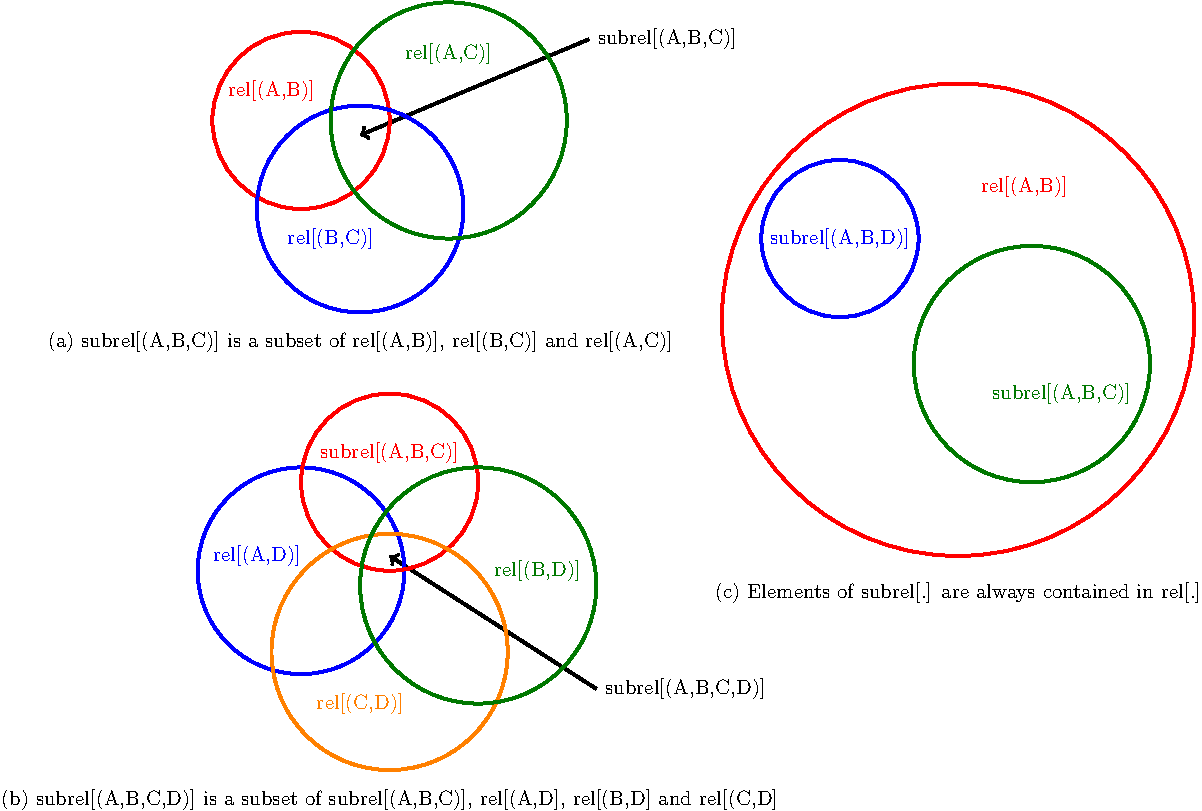
\includegraphics[width=0.5\paperwidth]{E:/Documents/TUM/THESIS/thesisCOD_Ha/figures/rel_example}
\end{figure}

\clearpage
    %%%%%%%%%%%%%%%%%%%%%%%%%%%%%%%%%%%%%%%%%%%%%%%
\chapter{Conclusion} \label{chap:conclusion}
%%%%%%%%%%%%%%%%%%%%%%%%%%%%%%%%%%%%%%%%%%%%%%%

In this thesis, we have shown combinatorial proofs for an existence
of new gaps for 3 generalized combination networks. The $\left(\epsilon=1,\ell=1\right)-\mathcal{N}_{h=3,r,s=4}$
network with $t=2$ has been studied in \cite{Wachter-Zeh:2018,Etzion:2016,Zhang:2019,Etzion:2018}
but no general gap was found. We also got computational results for
this network with 89 two-dimensional subspaces of $\ensuremath{\mathbb{F}}_{2}^{6}$,
which is better the constructed set of 51 two-dimensional subspaces
of $\ensuremath{\mathbb{F}}_{2}^{6}$ found in \cite{Wachter-Zeh:2018}.

In Chapter 5, by applying the Local lemma, we stated that there is
an $r_{\mathrm{max,vector}}\in\Omega\left(q^{t^{2}/2+\mathcal{O}\left(t\right)}\right)$
such that for any $r\leq r_{\mathrm{max,vector}}$ there exists a
vector solution for the $\left(\epsilon=1,l=1\right)-\mathcal{N}_{h=3,r,s=4}$
network. The optimal scalar solution for such network exists, when
$r\leq\mathcal{O}\left(q_{\mathrm{s}}^{2}\right)$. Therefore, a lower
bound on the gap $g_{\mathrm{lower\,bound}}=q^{t^{2}/4+\mathcal{O}(t)}$
exists for the $\left(1,1\right)-\mathcal{N}_{3,r,4}$ network. Similarly
we derived the gaps for the $\left(\epsilon=1,\ell=1\right)-\mathcal{N}_{h,r,s}$
network, the $\left(\epsilon>1,\ell=1\right)-\mathcal{N}_{h,r,s}$
network and the $\left(\epsilon=1,\ell>1\right)-\mathcal{N}_{h=2\ell,r,s=2\ell+1}$
network, respectively with $g_{\mathrm{lower\,bound}}=q^{\frac{\alpha-h+1}{\left(\alpha-1\right)\left(\alpha-h+2\right)\left(h-2\right)}t^{2}+\mathcal{O}(t)}$,
$g_{\mathrm{lower\,bound}}=q^{\frac{\epsilon\left(\alpha-h+\epsilon\right)}{\left(\alpha-1\right)\left(\alpha-h+\epsilon+1\right)\left(h-\epsilon-1\right)}t^{2}+\mathcal{O}(t)}$
and $g_{\mathrm{lower\,bound}}=q^{t^{2}/2\ell+\mathcal{O}(t)}$. A
comparison with known results can be found in Table \ref{tab:New-gap-found}
and Table \ref{tab:r_over_t}.

In Chapter 6, we introduced 4 different approaches in computing vector
solutions that outperform the optimal scalar solution for the $\left(\epsilon=1,\ell=1\right)-\mathcal{N}_{h=3,r,s=4}$
network with $t=2$. All approaches gave us such vector solutions,
and the Algorithm \ref{alg:Increasing-Method} called ``Increasing
Method'' generated the best result among 4 approaches. The best result
is about 2 times 42 results of the optimal scalar solution, i.e. we
found $r_{vector}=89$. When we mention the results of the optimal
scalar solution, it means that such a solution exists if and only
if $r_{scalar}\leq42$. However, our computational result of $r_{vector}$
is still less than the upper bound of $\mathcal{A}_{2}\left(6,4,3;2\right)$
in \cite{Etzion:2018}. Hence, we can only conclude $89\leq\mathcal{A}_{2}\left(6,4,3;2\right)\leq126$
for the $\left(\epsilon=1,\ell=1\right)-\mathcal{N}_{h=3,r,s=4}$
network with $t=2$. This motivates an open research to find a computational
method for generating a vector solution of 126 two-dimensional subspaces
of $\ensuremath{\mathbb{F}}_{2}^{6}$. At the time writing this thesis,
the best computational result is $r_{vector}=121$ stated in \cite{Etzion:2018}.
In Appendix \ref{sec:89-Two-Dimensional-Subspaces}, we listed one
of 2 different sets of our 89 two-dimensional subspaces of $\ensuremath{\mathbb{F}}_{2}^{6}$,
which are slightly different in 2 subspaces. We also find an interesting
result that there are $\left|U(2,6)\right|=715$ matrices whose different
row spaces among $\left|M(2,6)\right|=4096$ matrices over $\ensuremath{\mathbb{F}}_{2}^{6}$.
Furthermore, we used the Algorithm \ref{alg:Increasing-Method} and
got $r_{vector}=166$ for $t=3$ by Construction 1, which is better
than the optimal scalar solution existing if and only $r_{scalar}\leq146$.
This computational result was not found in any previous studies in
our scope of knowledge. For the $\left(\epsilon=1,\ell=1\right)-\mathcal{N}_{h=3,r,s=4}$
network with $t=3$, we therefore state a new bound $166\leq\mathcal{A}_{2}\left(9,6,3;2\right)\leq537$.
In Appendix \ref{sec:166-Three-Dimensional-Subspaces}, we wrote down
one of 18 found variants of 166 three-dimensional subspaces of $\ensuremath{\mathbb{F}}_{2}^{9}$.
From $\left|M(3,6)\right|=262144$ matrices, we found $\left|U(3,6)\right|=2110$
matrices whose different row spaces. All of computational results
in this study was listed in Table \ref{tab:r_over_t}. 

Another open research is to study a gap for the general network $\left(\epsilon,\ell\right)-\mathcal{N}_{h,r,s}$
with $\left(\epsilon>1,\ell>1\right)$ or $\left(\epsilon=1,\ell>1\right)$
for any $\alpha\geq1$. The most challenging problem for such research
is to define the optimal scalar solution for such network.

\clearpage  
    %%%%%%%%%%%%%%%%%%%%%%%%%%%%%%%%%%%%%%%%%%%%%%%
\chapter{Appendices} \label{chap:appendix}
%%%%%%%%%%%%%%%%%%%%%%%%%%%%%%%%%%%%%%%%%%%%%%%

\section{Proofs of Theorem \ref{theo:e2l1_r_max_vector}, Theorem \ref{theo:e2l1_r_max_scalar}
and Corollary \ref{cor:e2l1_gap} \label{app:proofs_e2l1}}
\begin{proof}[Proof of Theorem \vref{theo:e2l1_r_max_vector}]
 As in Section \vref{sec:e1l1_nw}, there exists a vector solution
for the $\left(\epsilon>1,\ell=1\right)-\mathcal{N}_{h,r,s}$ network
if
\[
\mathrm{rk}\left[\begin{array}{c}
\boldsymbol{A}^{\left(r_{1}\right)}\\
\vdots\\
\boldsymbol{A}^{\left(r_{\alpha}\right)}
\end{array}\right]\geq\left(h-\epsilon\right)t.
\]
Similar to Lemma \ref{lem:p_e1l1}, we have $p\in\Theta\left(q^{\left(\epsilon h-\epsilon\alpha-\epsilon^{2}\right)t^{2}+\mathcal{O}(t)}\right)$.
And there is no difference for $d$, we then have $r_{\mathrm{max,vector}}\in\Omega\left(q^{\frac{\epsilon\left(h-\alpha-\epsilon\right)}{1-\alpha}t^{2}+\mathcal{O}(t)}\right)$
following to the Local lemma \ref{thm:LLL}.
\end{proof}
%
\begin{proof}[Proof of Theorem \vref{theo:e2l1_r_max_scalar}]
 As in the proof of Theorem \ref{theo:r_scalar_e1l1}, there exists
a scalar solution for the $\left(\epsilon>1,\ell=1\right)-\mathcal{N}_{h,r,s}$
network if

\begin{eqnarray*}
 & r & \leq\left(\alpha-1\right)\stackrel[i=0]{h-\epsilon-2}{\prod}\frac{q_{\mathrm{s}}^{\alpha}-q_{\mathrm{s}}^{i}}{q_{\mathrm{s}}^{h-\epsilon-1}-q_{\mathrm{s}}^{i}}\approx\left(\alpha-1\right)\left(q_{\mathrm{s}}^{\left(\alpha-h+\epsilon+1\right)\left(h-\epsilon-1\right)}\right)\\
\Rightarrow & r_{\mathrm{max,scalar}} & \in\mathcal{O}\left(q_{\mathrm{s}}^{\left(\alpha-h+\epsilon+1\right)\left(h-\epsilon-1\right)}\right).
\end{eqnarray*}

Hence, there exists such $r_{\mathrm{max,scalar}}$ such that for
any $r\leq r_{\mathrm{max,scalar}}$there exists a scalar solution
for the network.
\end{proof}
%
\begin{proof}[Proof of Corollary \vref{cor:e2l1_gap}]
 The gap follows by applying Section \ref{subsec:Comparison-between-scalar-and-vector-sol}
with Theorem \vref{theo:e2l1_r_max_vector} and Theorem \vref{theo:e2l1_r_max_scalar}.
\end{proof}

\section{89 Two-Dimensional Subspaces of $\ensuremath{\mathbb{F}}_{2}^{6}$
for the $\left(\epsilon=1,\ell=1\right)-\mathcal{N}_{h=3,r,s=4}$
Network \label{sec:89-Two-Dimensional-Subspaces}}

By applying Algorithm \vref{alg:Increasing-Method} with details mentioned
in Section (\ref{sec:Main-Approach}), we computed the following 89
subspaces of $\ensuremath{\mathbb{F}}_{2}^{6}$ for our vector solution
for the $\left(\epsilon=1,\ell=1\right)-\mathcal{N}_{h=3,r,s=4}$
network, which are equivalently to 89 intermediate nodes in the middle
layer of the network.

\begin{lstlisting}
[1 0 0 0 0 0] [1 0 0 0 0 0] [0 0 1 0 0 0] [0 0 0 1 0 0] 
[0 1 0 0 0 0] [0 0 1 0 0 0] [0 0 0 0 0 1] [0 0 0 0 1 0] 

[1 0 0 0 1 0] [1 0 0 0 0 0] [1 0 0 0 0 0] [0 1 0 0 1 0] 
[0 0 0 0 0 1] [0 0 1 0 1 0] [0 0 0 1 0 1] [0 0 0 1 0 0] 

[0 1 0 0 0 1] [0 0 1 0 0 1] [0 0 0 1 0 1] [1 1 1 0 0 0] 
[0 0 1 0 0 0] [0 0 0 1 0 0] [0 0 0 0 1 0] [0 0 0 0 1 0] 

[1 0 1 0 0 0] [1 0 1 0 0 0] [1 0 1 0 0 0] [1 0 0 1 0 0] 
[1 0 0 1 0 0] [0 1 0 1 0 0] [0 0 0 1 1 0] [1 0 0 0 0 1] 

[1 0 0 0 1 1] [1 0 0 0 1 0] [1 0 0 0 0 1] [0 1 1 1 0 0] 
[0 0 0 1 0 0] [1 0 0 0 0 1] [0 1 0 1 0 0] [0 0 0 0 1 0] 

[0 1 1 0 0 0] [0 1 1 0 0 0] [0 1 0 0 0 1] [0 1 0 0 0 0] 
[0 1 0 0 1 0] [0 0 0 1 0 1] [0 0 1 1 0 0] [0 0 1 1 1 0] 

[0 0 1 1 1 0] [0 0 1 1 0 0] [1 1 1 0 0 0] [1 1 1 0 0 0] 
[0 0 0 0 0 1] [0 0 0 0 1 1] [1 0 0 0 1 0] [0 1 0 1 0 0] 

[1 1 0 1 0 0] [1 1 0 0 1 0] [1 1 0 0 1 0] [1 1 0 0 0 1] 
[0 1 0 0 1 0] [0 1 0 1 0 0] [0 1 0 0 0 1] [1 0 0 1 0 0] 

[1 1 0 0 0 0] [1 1 0 0 0 0] [1 0 1 1 1 0] [1 0 1 1 0 0] 
[1 0 1 0 0 1] [0 0 0 1 1 1] [0 0 0 0 0 1] [0 1 0 0 0 1] 

[1 0 1 1 0 0] [1 0 1 0 1 1] [1 0 1 0 1 1] [1 0 0 1 1 0] 
[0 0 1 0 0 1] [0 1 0 0 0 0] [0 0 0 1 0 0] [0 0 0 0 1 1] 

[1 0 0 0 0 1] [0 1 1 0 0 1] [0 1 0 1 1 1] [0 0 1 1 0 1] 
[0 1 0 1 1 0] [0 0 1 0 1 0] [0 0 1 0 0 0] [0 0 1 0 1 0] 

[0 0 1 1 0 0] [1 1 1 1 1 0] [1 1 1 1 0 0] [1 1 1 0 1 0] 
[0 0 1 0 1 1] [0 0 0 0 0 1] [0 1 0 0 0 1] [0 0 1 0 0 1] 

[1 1 1 0 0 1] [1 1 0 1 1 0] [1 1 0 1 0 1] [1 1 0 1 0 0] 
[0 0 0 1 1 0] [1 0 1 0 0 0] [0 1 1 0 0 0] [1 0 0 0 1 1] 

[1 1 0 1 0 0] [1 1 0 0 1 1] [1 1 0 0 1 1] [1 1 0 0 1 0] 
[0 0 1 1 0 1] [0 1 1 0 0 0] [0 0 1 1 0 0] [0 1 1 1 0 0] 

[1 1 0 0 0 1] [1 1 0 0 0 1] [1 0 1 1 0 0] [1 0 1 1 0 0] 
[1 0 1 0 1 0] [0 1 1 0 1 0] [0 1 0 1 0 1] [0 0 0 1 1 1] 

[1 0 1 0 1 0] [1 0 1 0 0 1] [1 0 1 0 0 1] [1 0 0 1 1 0] 
[0 1 0 1 1 0] [0 1 1 1 0 0] [0 1 0 1 0 1] [0 1 0 1 0 1] 

[1 0 0 1 0 1] [1 0 0 1 0 1] [1 0 0 0 0 1] [0 1 1 1 0 1] 
[0 1 1 0 1 0] [0 0 1 0 1 1] [0 1 1 1 1 0] [0 0 0 1 1 0] 

[0 1 1 0 1 1] [0 1 1 0 0 1] [0 1 0 1 0 1] [0 1 0 0 1 1] 
[0 1 0 1 0 0] [0 1 0 1 1 0] [0 0 1 0 1 1] [0 0 1 1 1 0] 

[1 1 1 1 1 0] [1 1 1 1 1 0] [1 1 1 1 0 0] [1 1 1 0 0 1] 
[0 0 0 1 0 1] [0 0 0 0 1 1] [0 1 0 0 1 1] [0 0 1 1 1 0] 

[1 1 0 1 1 0] [1 1 0 1 1 0] [1 1 0 1 0 1] [1 1 0 1 0 0] 
[1 0 1 0 0 1] [0 0 1 1 0 1] [0 0 1 0 1 1] [0 1 1 0 1 1] 

[1 1 0 0 1 1] [1 1 0 0 0 1] [1 0 1 1 0 1] [1 0 1 0 1 0] 
[0 0 1 1 1 0] [1 0 1 1 1 0] [0 1 1 0 1 0] [0 1 0 1 1 1] 

[1 0 0 1 1 1] [1 0 0 1 1 1] [1 1 1 0 1 0] [1 1 1 0 1 0] 
[0 1 1 1 0 0] [0 1 1 0 1 0] [1 0 1 1 0 1] [1 0 0 1 1 1] 

[1 1 0 1 1 0] 
[1 0 1 1 0 1]
\end{lstlisting}


\section{166 Three-Dimensional Subspaces of $\ensuremath{\mathbb{F}}_{2}^{9}$
for the $\left(\epsilon=1,\ell=1\right)-\mathcal{N}_{h=3,r,s=4}$
Network \label{sec:166-Three-Dimensional-Subspaces}}

By applying Algorithm \vref{alg:Increasing-Method} with details mentioned
in Section (\ref{sec:Main-Approach}), we computed the following 166
subspaces of $\ensuremath{\mathbb{F}}_{2}^{9}$ for our vector solution
for the $\left(\epsilon=1,\ell=1\right)-\mathcal{N}_{h=3,r,s=4}$
network, which are equivalently to 166 intermediate nodes in the middle
layer of the network. A vector solution over $\ensuremath{\mathbb{F}}_{2}^{9}$
for the $\left(\epsilon=1,\ell=1\right)-\mathcal{N}_{h=3,r,s=4}$
network has not yet been studied in any other studies.

\begin{lstlisting}
[1 0 0 0 0 1 0 0 0] [1 0 0 0 0 0 1 0 0] 
[0 1 0 0 0 0 0 1 0] [0 1 0 0 0 0 0 0 1] 
[0 0 1 0 0 0 0 0 0] [0 0 1 0 0 0 0 0 0] 

[1 0 0 1 0 1 0 1 0] [1 0 0 1 1 0 1 0 1] 
[0 1 0 1 0 0 1 0 0] [0 1 0 1 0 1 0 0 0] 
[0 0 1 0 0 0 0 1 1] [0 0 1 0 0 0 0 1 0] 

[1 0 0 1 0 0 1 0 0] [1 0 0 0 0 1 1 1 0] 
[0 1 0 0 1 1 0 1 0] [0 1 0 0 0 0 0 1 1] 
[0 0 1 0 0 0 0 0 1] [0 0 1 0 0 0 0 0 0] 

[1 0 0 1 0 1 0 1 0] [1 0 0 0 0 1 1 0 1] 
[0 1 0 0 1 1 1 0 0] [0 1 0 0 0 0 1 1 0] 
[0 0 1 0 1 0 0 0 1] [0 0 1 0 0 0 0 0 0] 

[1 0 0 1 1 0 0 0 0] [1 0 0 1 0 1 0 1 0] 
[0 1 0 0 0 0 0 1 0] [0 1 0 0 1 0 1 1 0] 
[0 0 1 0 0 0 0 0 0] [0 0 1 0 0 0 1 0 1] 

[1 0 0 1 0 0 0 1 0] [1 0 0 1 0 0 0 0 1] 
[0 1 0 0 0 1 0 0 0] [0 1 0 0 0 0 1 0 0] 
[0 0 1 0 0 0 0 0 0] [0 0 1 0 0 0 0 0 0] 

[1 0 0 1 1 0 1 0 0] [1 0 0 1 0 0 0 0 0] 
[0 1 0 1 0 1 0 1 0] [0 1 0 0 1 0 0 0 1] 
[0 0 1 0 0 0 0 1 1] [0 0 1 0 0 0 0 0 0] 

[1 0 0 1 0 0 0 0 0] [1 0 0 1 0 0 0 0 0] 
[0 1 0 0 1 0 0 0 0] [0 1 0 0 0 1 0 0 0] 
[0 0 1 0 0 1 0 0 0] [0 0 1 0 0 0 1 0 0] 

[1 0 0 1 0 0 0 0 0] [1 0 0 0 1 0 0 1 0] 
[0 1 0 0 0 0 1 0 0] [0 1 0 0 0 0 0 0 1] 
[0 0 1 0 0 0 0 1 0] [0 0 1 0 0 0 0 0 0] 

[1 0 0 1 1 0 0 1 0] [1 0 0 0 1 0 0 0 0] 
[0 1 0 1 0 0 1 0 1] [0 1 0 0 0 1 0 0 0] 
[0 0 1 0 1 1 0 0 1] [0 0 1 0 0 0 1 0 0] 

[1 0 0 0 1 0 0 0 0] [1 0 0 1 1 0 1 0 0] 
[0 1 0 0 0 0 1 1 0] [0 1 0 1 0 0 0 1 0] 
[0 0 1 0 0 0 0 0 0] [0 0 1 1 0 0 0 0 1] 

[1 0 0 0 0 1 0 1 0] [1 0 0 1 1 0 0 0 1] 
[0 1 0 0 0 0 1 0 0] [0 1 0 0 1 1 0 0 0] 
[0 0 1 0 0 0 0 0 0] [0 0 1 0 0 0 1 1 1] 

[1 0 0 1 1 0 1 0 0] [1 0 0 1 0 0 0 1 1] 
[0 1 0 0 1 1 0 0 0] [0 1 0 0 1 0 1 0 0] 
[0 0 1 0 1 0 0 0 1] [0 0 1 0 0 1 0 0 0] 

[1 0 0 1 1 0 1 0 0] [1 0 0 0 0 0 1 0 0] 
[0 1 0 0 0 1 1 1 1] [0 1 0 0 0 0 0 1 0] 
[0 0 1 0 0 0 0 0 0] [0 0 1 0 0 0 0 0 1] 

[1 0 0 0 0 1 0 1 0] [1 0 0 1 1 0 1 1 0] 
[0 1 0 0 0 1 0 0 1] [0 1 0 1 0 1 0 0 0] 
[0 0 1 0 0 0 1 0 0] [0 0 1 0 1 0 0 0 1] 

[1 0 0 1 0 0 0 1 0] [1 0 0 1 1 0 0 1 1] 
[0 1 0 1 0 0 0 0 1] [0 1 0 1 0 0 1 0 0] 
[0 0 1 0 1 1 0 0 0] [0 0 1 0 0 1 0 0 0] 

[1 0 0 1 0 1 0 0 1] [1 0 0 1 1 0 1 1 0] 
[0 1 0 1 0 0 0 1 0] [0 1 0 0 1 1 0 0 0] 
[0 0 1 0 1 0 1 0 1] [0 0 1 0 0 0 1 0 1] 

[1 0 0 1 0 1 0 0 1] [1 0 0 1 0 1 0 0 1] 
[0 1 0 0 1 1 1 0 0] [0 1 0 0 1 1 0 1 0] 
[0 0 1 0 0 0 1 1 0] [0 0 1 0 1 0 1 0 0] 

[1 0 0 1 0 1 0 1 0] [1 0 0 1 1 0 1 0 1] 
[0 1 0 0 1 0 0 0 1] [0 1 0 0 0 0 0 0 0] 
[0 0 1 0 0 1 1 0 0] [0 0 1 0 0 0 0 0 0] 

[1 0 0 1 0 1 0 0 1] [1 0 0 1 1 0 0 1 0] 
[0 1 0 0 1 0 1 0 1] [0 1 0 1 0 1 1 0 0] 
[0 0 1 0 0 1 0 1 0] [0 0 1 0 1 1 0 0 1] 

[1 0 0 1 0 1 0 0 0] [1 0 0 1 1 0 0 1 0] 
[0 1 0 0 1 0 0 0 0] [0 1 0 0 1 1 0 0 0] 
[0 0 1 0 0 0 0 1 0] [0 0 1 0 1 0 1 0 0] 

[1 0 0 1 1 0 0 1 0] [1 0 0 1 0 0 1 0 0] 
[0 1 0 0 1 0 1 0 0] [0 1 0 0 1 1 0 0 0] 
[0 0 1 0 1 0 0 0 1] [0 0 1 0 0 0 0 0 0] 

[1 0 0 1 0 0 0 1 0] [1 0 0 1 1 0 1 0 1] 
[0 1 0 0 1 0 0 0 0] [0 1 0 0 1 1 0 0 0] 
[0 0 1 0 0 0 0 0 1] [0 0 1 0 1 0 0 1 0] 

[1 0 0 1 1 0 0 0 1] [1 0 0 1 1 0 0 0 1] 
[0 1 0 1 0 1 1 1 0] [0 1 0 1 0 1 0 0 0] 
[0 0 1 0 0 0 0 0 0] [0 0 1 1 0 0 1 0 0] 

[1 0 0 1 1 0 0 0 1] [1 0 0 1 0 0 0 1 1] 
[0 1 0 1 0 0 0 1 0] [0 1 0 0 1 1 0 1 0] 
[0 0 1 0 1 1 0 0 0] [0 0 1 0 1 0 1 0 0] 

[1 0 0 1 1 0 0 0 1] [1 0 0 1 1 0 0 0 1] 
[0 1 0 0 1 1 0 1 0] [0 1 0 0 1 0 1 1 0] 
[0 0 1 0 0 0 1 0 0] [0 0 1 0 0 1 0 0 0] 

[1 0 0 0 1 1 0 0 0] [1 0 0 1 0 1 0 0 0] 
[0 1 0 0 1 0 0 0 1] [0 1 0 1 0 0 0 1 1] 
[0 0 1 0 0 0 0 0 0] [0 0 1 0 1 0 1 1 0] 

[1 0 0 0 1 0 1 0 0] [1 0 0 1 1 0 1 0 0] 
[0 1 0 0 0 1 0 0 0] [0 1 0 1 0 1 0 0 0] 
[0 0 1 0 0 0 0 0 1] [0 0 1 0 0 0 1 1 1] 

[1 0 0 1 0 0 0 0 0] [1 0 0 1 1 0 0 0 1] 
[0 1 0 0 1 1 0 1 0] [0 1 0 1 0 1 0 1 0] 
[0 0 1 0 0 1 1 0 0] [0 0 1 0 1 1 1 0 0] 

[1 0 0 1 1 0 0 0 1] [1 0 0 1 0 0 0 0 0] 
[0 1 0 1 0 1 0 1 0] [0 1 0 0 1 0 1 0 0] 
[0 0 1 0 1 0 1 1 0] [0 0 1 0 1 0 0 1 1] 

[1 0 0 1 1 0 0 0 0] [1 0 0 1 1 0 0 0 0] 
[0 1 0 1 0 1 1 0 0] [0 1 0 1 0 1 0 1 0] 
[0 0 1 0 0 1 0 0 1] [0 0 1 0 0 1 1 0 0] 

[1 0 0 1 1 0 0 0 0] [1 0 0 1 0 0 0 0 0] 
[0 1 0 1 0 1 0 0 1] [0 1 0 0 1 1 1 0 1] 
[0 0 1 1 0 0 0 1 0] [0 0 1 0 1 0 0 1 0] 

[1 0 0 0 1 0 0 0 0] [1 0 0 1 0 0 0 0 0] 
[0 1 0 0 0 0 1 0 0] [0 1 0 0 0 1 1 0 1] 
[0 0 1 0 0 0 0 1 1] [0 0 1 0 0 0 1 1 0] 

[1 0 0 1 1 0 0 0 0] [1 0 0 1 0 0 0 0 0] 
[0 1 0 1 0 0 1 0 1] [0 1 0 0 1 1 0 0 1] 
[0 0 1 1 0 0 0 1 0] [0 0 1 0 0 1 1 1 0] 

[1 0 0 0 0 1 1 0 0] [1 0 0 1 0 1 0 0 0] 
[0 1 0 0 0 1 0 1 0] [0 1 0 1 0 0 1 0 1] 
[0 0 1 0 0 0 0 0 0] [0 0 1 0 1 0 0 1 1] 

[1 0 0 1 0 1 0 0 1] [1 0 0 1 0 1 0 0 1] 
[0 1 0 1 0 0 1 1 0] [0 1 0 1 0 0 1 1 0] 
[0 0 1 0 1 1 1 0 0] [0 0 1 0 1 1 0 1 0] 

[1 0 0 0 1 1 1 1 0] [1 0 0 1 1 0 0 1 0] 
[0 1 0 0 0 1 0 0 1] [0 1 0 1 0 1 0 0 1] 
[0 0 1 0 0 0 0 0 0] [0 0 1 0 0 1 1 0 0] 

[1 0 0 1 1 0 0 1 1] [1 0 0 0 1 0 1 0 0] 
[0 1 0 1 0 1 1 0 1] [0 1 0 0 1 0 0 1 1] 
[0 0 1 0 0 0 0 0 0] [0 0 1 0 0 1 0 0 0] 

[1 0 0 0 1 1 1 0 0] [1 0 0 0 0 0 1 1 0] 
[0 1 0 0 0 0 1 1 0] [0 1 0 0 0 0 1 0 1] 
[0 0 1 0 0 0 0 0 1] [0 0 1 0 0 0 0 0 0] 

[1 0 0 0 1 1 0 1 0] [1 0 0 1 0 0 1 1 0] 
[0 1 0 0 0 1 1 0 0] [0 1 0 1 0 0 0 0 1] 
[0 0 1 0 0 0 0 0 1] [0 0 1 0 1 1 0 1 0] 

[1 0 0 1 0 1 1 0 1] [1 0 0 0 1 1 0 0 1] 
[0 1 0 0 1 0 1 1 0] [0 1 0 0 1 0 0 1 0] 
[0 0 1 0 0 0 0 0 0] [0 0 1 0 0 0 1 0 0] 

[1 0 0 0 1 1 0 0 1] [1 0 0 0 1 1 1 0 0] 
[0 1 0 0 0 1 0 1 0] [0 1 0 0 1 0 0 1 0] 
[0 0 1 0 0 0 1 0 0] [0 0 1 0 0 0 1 0 1] 

[1 0 0 0 1 1 0 0 0] [1 0 0 1 0 1 1 0 0] 
[0 1 0 0 1 0 1 0 1] [0 1 0 1 0 0 0 0 1] 
[0 0 1 0 0 0 1 1 0] [0 0 1 0 0 0 1 1 0] 

[1 0 0 0 1 1 1 0 0] [1 0 0 1 1 0 0 1 0] 
[0 1 0 0 0 1 0 0 1] [0 1 0 0 1 0 0 0 1] 
[0 0 1 0 0 0 1 1 0] [0 0 1 0 0 1 1 1 0] 

[1 0 0 0 1 1 0 0 0] [1 0 0 1 1 0 0 1 0] 
[0 1 0 0 1 0 1 0 0] [0 1 0 0 0 1 1 1 0] 
[0 0 1 0 1 0 0 0 1] [0 0 1 0 0 1 0 0 1] 

[1 0 0 1 0 1 1 0 0] [1 0 0 1 0 1 0 1 1] 
[0 1 0 0 0 1 0 1 0] [0 1 0 1 0 0 1 0 0] 
[0 0 1 0 0 0 1 0 1] [0 0 1 0 1 0 0 0 0] 

[1 0 0 1 0 0 1 0 1] [1 0 0 1 1 0 0 0 1] 
[0 1 0 1 0 0 0 1 0] [0 1 0 1 0 1 1 0 0] 
[0 0 1 0 1 1 1 0 0] [0 0 1 0 1 0 0 1 0] 

[1 0 0 1 1 0 0 0 1] [1 0 0 0 1 1 0 1 0] 
[0 1 0 1 0 0 1 0 0] [0 1 0 0 1 0 1 0 0] 
[0 0 1 0 0 1 0 1 1] [0 0 1 0 0 1 0 0 1] 

[1 0 0 1 0 0 1 0 0] [1 0 0 1 1 0 1 0 0] 
[0 1 0 1 0 0 0 1 1] [0 1 0 0 0 1 0 0 0] 
[0 0 1 0 1 1 0 0 1] [0 0 1 0 0 0 0 1 0] 

[1 0 0 1 1 0 0 0 0] [1 0 0 1 1 0 0 0 0] 
[0 1 0 1 0 0 0 1 0] [0 1 0 1 0 0 0 0 1] 
[0 0 1 0 0 1 0 0 0] [0 0 1 0 0 0 0 1 0] 

[1 0 0 0 1 1 0 0 1] [1 0 0 1 1 1 0 1 0] 
[0 1 0 0 1 0 1 0 0] [0 1 0 0 0 0 0 1 1] 
[0 0 1 0 0 1 0 1 0] [0 0 1 0 0 0 0 0 0] 

[1 0 0 1 0 1 0 0 1] [1 0 0 1 0 1 0 0 1] 
[0 1 0 1 0 0 1 0 0] [0 1 0 0 1 0 0 1 1] 
[0 0 1 1 0 0 0 1 0] [0 0 1 0 0 0 1 0 0] 

[1 0 0 1 0 1 0 1 0] [1 0 0 1 1 1 0 0 0] 
[0 1 0 0 0 1 0 0 1] [0 1 0 0 0 1 0 0 1] 
[0 0 1 0 0 0 0 0 0] [0 0 1 0 0 0 1 0 0] 

[1 0 0 1 0 1 0 0 1] [1 0 0 1 1 1 0 0 0] 
[0 1 0 0 1 0 1 0 0] [0 1 0 0 0 0 1 0 1] 
[0 0 1 0 0 0 0 0 0] [0 0 1 0 0 0 0 1 0] 

[1 0 0 1 1 0 0 0 0] [1 0 0 1 0 1 0 0 0] 
[0 1 0 1 0 1 0 1 1] [0 1 0 1 0 0 1 0 0] 
[0 0 1 1 0 0 1 0 0] [0 0 1 0 0 0 0 1 0] 

[1 0 0 1 0 1 0 0 0] [1 0 0 0 1 0 0 1 1] 
[0 1 0 1 0 0 0 0 1] [0 1 0 0 0 1 1 1 0] 
[0 0 1 0 1 0 0 0 0] [0 0 1 0 0 0 0 0 0] 

[1 0 0 1 1 0 0 0 0] [1 0 0 1 1 0 1 0 0] 
[0 1 0 1 0 0 0 1 1] [0 1 0 1 0 1 0 0 1] 
[0 0 1 0 0 1 1 1 0] [0 0 1 0 1 0 0 1 1] 

[1 0 0 1 0 0 1 0 1] [1 0 0 1 0 0 1 0 0] 
[0 1 0 0 1 0 0 0 0] [0 1 0 1 0 0 0 0 1] 
[0 0 1 0 0 1 0 0 0] [0 0 1 0 0 0 0 1 0] 

[1 0 0 1 0 0 1 0 0] [1 0 0 1 1 0 0 1 0] 
[0 1 0 0 1 0 0 0 0] [0 1 0 1 0 1 0 0 0] 
[0 0 1 0 0 1 0 1 0] [0 0 1 0 0 0 1 0 0] 

[1 0 0 1 1 0 0 1 0] [1 0 0 1 0 1 0 0 0] 
[0 1 0 0 1 0 1 0 1] [0 1 0 0 1 0 1 1 0] 
[0 0 1 0 0 0 0 0 0] [0 0 1 0 0 0 0 1 1] 

[1 0 0 1 0 0 0 1 0] [1 0 0 1 0 0 0 1 0] 
[0 1 0 0 1 0 0 0 0] [0 1 0 0 0 1 0 0 0] 
[0 0 1 0 0 1 0 0 1] [0 0 1 0 0 0 1 0 1] 

[1 0 0 1 1 0 0 0 0] [1 0 0 1 1 0 0 0 0] 
[0 1 0 1 0 1 0 0 0] [0 1 0 1 0 0 1 0 0] 
[0 0 1 1 0 0 0 0 1] [0 0 1 1 0 0 0 0 1] 

[1 0 0 0 1 0 0 0 0] [1 0 0 1 1 0 1 0 0] 
[0 1 0 0 0 1 1 0 1] [0 1 0 0 1 0 0 1 0] 
[0 0 1 0 0 0 1 1 0] [0 0 1 0 0 1 0 0 0] 

[1 0 0 1 1 0 0 0 0] [1 0 0 1 1 1 0 0 0] 
[0 1 0 0 0 0 1 1 0] [0 1 0 1 0 0 1 0 1] 
[0 0 1 0 0 0 1 0 1] [0 0 1 0 1 0 1 1 0] 

[1 0 0 1 0 0 0 0 0] [1 0 0 1 0 0 0 0 0] 
[0 1 0 0 1 0 0 1 0] [0 1 0 0 0 1 1 0 0] 
[0 0 1 0 1 0 0 0 1] [0 0 1 0 0 1 0 0 1] 

[1 0 0 1 1 1 1 0 0] [1 0 0 1 0 1 1 1 0] 
[0 1 0 1 0 0 1 1 1] [0 1 0 1 0 0 0 0 1] 
[0 0 1 0 0 0 0 0 0] [0 0 1 0 0 0 0 0 0] 

[1 0 0 1 1 1 1 0 0] [1 0 0 1 1 1 1 0 0] 
[0 1 0 1 0 0 0 1 0] [0 1 0 1 0 0 0 0 1] 
[0 0 1 0 1 0 0 0 1] [0 0 1 0 0 1 0 1 0] 

[1 0 0 0 1 1 1 0 0] [1 0 0 1 0 1 1 0 0] 
[0 1 0 0 0 0 1 0 1] [0 1 0 0 0 1 0 0 1] 
[0 0 1 0 0 0 0 0 0] [0 0 1 0 0 0 0 1 0] 

[1 0 0 1 0 1 1 0 0] [1 0 0 0 1 1 0 0 1] 
[0 1 0 0 0 0 1 1 1] [0 1 0 0 0 1 1 0 0] 
[0 0 1 0 0 0 0 0 0] [0 0 1 0 0 0 0 0 0] 

[1 0 0 1 0 0 1 0 1] [1 0 0 1 1 1 1 0 1] 
[0 1 0 0 1 1 1 0 0] [0 1 0 0 0 1 0 1 0] 
[0 0 1 0 0 0 0 1 0] [0 0 1 0 0 0 0 0 0] 

[1 0 0 1 0 0 0 1 1] [1 0 0 1 1 0 1 0 0] 
[0 1 0 0 1 1 1 0 1] [0 1 0 0 1 1 0 0 1] 
[0 0 1 0 0 0 0 0 0] [0 0 1 0 0 1 0 1 0] 

[1 0 0 0 1 0 1 0 1] [1 0 0 0 1 0 1 0 0] 
[0 1 0 0 1 0 0 1 0] [0 1 0 0 1 0 0 0 1] 
[0 0 1 0 0 0 0 0 0] [0 0 1 0 0 1 0 0 0] 

[1 0 0 1 1 1 0 1 0] [1 0 0 1 0 1 0 0 0] 
[0 1 0 0 1 0 1 0 0] [0 1 0 1 0 0 0 1 0] 
[0 0 1 0 0 0 0 1 1] [0 0 1 1 0 0 0 0 1] 

[1 0 0 1 1 1 0 0 1] [1 0 0 1 1 1 0 0 1] 
[0 1 0 0 0 1 1 0 0] [0 1 0 1 0 0 1 0 0] 
[0 0 1 0 0 0 0 1 0] [0 0 1 1 0 0 0 1 0] 

[1 0 0 1 1 1 0 0 1] [1 0 0 1 1 1 0 0 0] 
[0 1 0 1 0 0 0 1 0] [0 1 0 1 0 0 1 0 0] 
[0 0 1 0 0 1 1 0 0] [0 0 1 0 0 1 0 1 0] 

[1 0 0 1 1 1 0 0 0] [1 0 0 1 1 1 0 0 0] 
[0 1 0 1 0 0 0 1 0] [0 1 0 1 0 0 0 0 1] 
[0 0 1 0 1 0 1 0 0] [0 0 1 0 1 0 1 0 0] 

[1 0 0 0 1 0 0 0 1] [1 0 0 1 1 1 0 0 0] 
[0 1 0 0 0 1 0 0 0] [0 1 0 0 1 0 1 0 0] 
[0 0 1 0 0 0 1 1 0] [0 0 1 0 1 0 0 1 0] 

[1 0 0 1 1 1 0 0 0] [1 0 0 1 1 1 0 0 0] 
[0 1 0 0 1 0 0 1 0] [0 1 0 0 1 0 0 0 1] 
[0 0 1 0 0 1 1 0 0] [0 0 1 0 0 0 1 1 0] 

[1 0 0 1 1 1 0 0 0] [1 0 0 1 1 0 1 0 0] 
[0 1 0 0 0 1 1 1 0] [0 1 0 1 0 0 0 1 1] 
[0 0 1 0 0 0 0 0 1] [0 0 1 0 1 1 0 1 0] 

[1 0 0 1 0 0 1 1 0] [1 0 0 1 0 0 1 0 1] 
[0 1 0 0 1 0 0 0 0] [0 1 0 0 0 1 0 1 1] 
[0 0 1 0 0 0 0 1 1] [0 0 1 0 0 0 0 0 0] 

[1 0 0 0 1 0 0 0 0] [1 0 0 1 1 0 0 1 0] 
[0 1 0 0 0 1 0 1 0] [0 1 0 0 0 1 0 0 0] 
[0 0 1 0 0 1 0 0 1] [0 0 1 0 0 0 0 1 1] 
\end{lstlisting}

\clearpage   
        
        \cleardoubleemptypage


% ########################################
% Appendix / Anhang:
% ########################################

% roman page numbering, starting with page number 1 (capitals)/ roemische Seitennummerierung beginnend mit Seite 1 (gross)
    \appendix
    \setcounter{page}{1}
    \pagenumbering{Roman}

        % Use IEEE DIN 1505 style for bibliography / Literaturverzeichnisses
        \bibliographystyle{ieeetransa}
        %\nocite{*}              % Include all references without checking / Alle References immer aufführen
        \bibliography{./refs/final_ref_bib}

\end{document}

%
% EOF!
%